\chapter{Propagating the Uncertainty from Stereo Images to the Cost Volume}\label{chap:propagating}
\todoroman{Citer la publication d'origine pour les figure (license CC BY)}
The previous chapter presented different methods for joining credal sets using a copula. In this chapter, we will see how those results can be applied to propagate the uncertainty in a stereo matching example. More specifically, we will use possibility distributions from chapter \ref{chap:representation_of_uncertainty} as uncertainty models on the intensity values of epipolar images used in stereo matching. We will then propagate the uncertainty from those images to the cost volume using results from section \ref{subsec:necessity_functions}. We will also show that propagating the uncertainty has the potential to improve the disparity map derived from the cost volume. This chapter takes up work and data already published \cite{malinowski_copulas_2022, malinowski_uncertainty_2023}.

It is important to note that in this disparity estimation problem, we only account for the uncertainty in our input image intensities, without considering the uncertainty in our cost function's ability to correctly identify the true disparity as its minimum. In other words, we do not account for the uncertainty arising from the difference between ``two patches are very similar'' and ``the pixels at the center of the patches are homologous''. We refer to figure \ref{fig:adherence_window} and the discussion in section \ref{sec:stereo_matching} regarding the adherence problem for more details. We focus in this chapter on the propagation of uncertainty. We will thus consider a stereo matching pipeline with a simple cost function and no SGM regularization. Indeed, propagating the uncertainty through a cost volume optimization is too complex and computationally expensive to be solved with this chapter's method. We will consider the different problem of uncertainty modelling with SGM regularization in the following chapter, chapter \ref{chap:epistemic_uncertainty}. 
\todoroman{Je remets ici les commentaires de Manue que j'ai commencé à intégrer:  1) le problème global que tu cherches à résoudre 2) les paramètres que tu vas utiliser pour le matching genre la fonction de coût considérer 3) les hypothèses simplificatrices. Général vers particulier. Et ensuite dans tous les cas il te faudra une sorte de synthèse à la fin de la section pour résumer les choix}

\section{Hypothesis for Uncertainty in Stereo Matching}\label{sec:sources_of_uncertainty}\commanue{J'ai toujours un pb avec ce titre, je le trouve super vague. Dans le cas précis, c'est les hypothèses/conditions que tu considères pour ton étude. C'est le contexte. Je me demande si il ne faudrait pas faire ressortir dans le texte, les hypothèses/conditions considérées ou alors faire un encart à la fin de la section pour que ce soit bien clair pour tout le monde le cadre d'utilisation. J'ai pas encore lu mais si tu as un cadre d'utilsiation, il faut que tu dises si c'est réaliste et applicable, ou au contrare très théorique et plus là pour donner une illustration posisble ce qu'on pourrait faire. ça manque peut-être dans l'intro d'expliquer l'applicabilité de ce cas d'utilisation et je te l'accorde je fais les remarques complètement dans le désordre. }

\subsection{Considered Stereo Matching Pipeline}
We consider the Sum of Absolute Differences (SAD) as our cost function, presented in section \ref{sec:cost_volume_computation}, and reminded here. Given patches $W_L\subset I_L$ and $W_R\subset I_R$ of the same shape with $n$ pixels (usually squares):
\begin{align}
    \SAD(W_L, W_R) = \sum_{(p_i, q_i)\in (W_L, W_R)}|I_L(p_i) - I_R(q_i)|\label{eq:SAD}
\end{align}
where $p_i$ and $q_i$ are pixels at the same position $i$ in their patch. For convenience purposes, we will refer to the Absolute Difference between two pixels as AD (when there is no sum involved). An illustration of the AD between pixels and SAD cost function can be found in Figure \ref{fig:SAD}.

\begin{remark}
    Although the SAD is not the best performing cost function for dense matching, it is both fast and easily parallelizable. It is often use for comparison in cost-based stereo algorithms \cite{hirschmuller_evaluation_2007, zbontar_stereo_2016}, or in other applications. Considering a simple cost function such as SAD is relevant for different reasons:
    \begin{itemize}
        \item Simple stereo matching algorithms are often used as a quick and easy method for estimating the disparity.
        \item Simple cost functions (such as SAD, ZNCC, \etc) considered here are still used in other problems, such as video compression for instance \cite{richardson_h264_2006}.
        \item As both stereo matching and uncertainty propagation can be complicated problems, considering a simple stereo algorithm allow us to remain (relatively) simple and didactic in our explanations. 
    \end{itemize}
\end{remark}

As stated previously, we will not consider in this chapter the use of Semi Global Matching (or similar regularization methods), as it necessitates many operations due to its recursive formulation and thus greatly increases complexity for the uncertainty propagation. We diverge from state-of-the-art methods to keep explanations as simple as possible, however the modeling of uncertainty for more advanced cost functions and SGM methods will be considered in chapter \ref{chap:epistemic_uncertainty}.


\begin{figure}
    \centering
    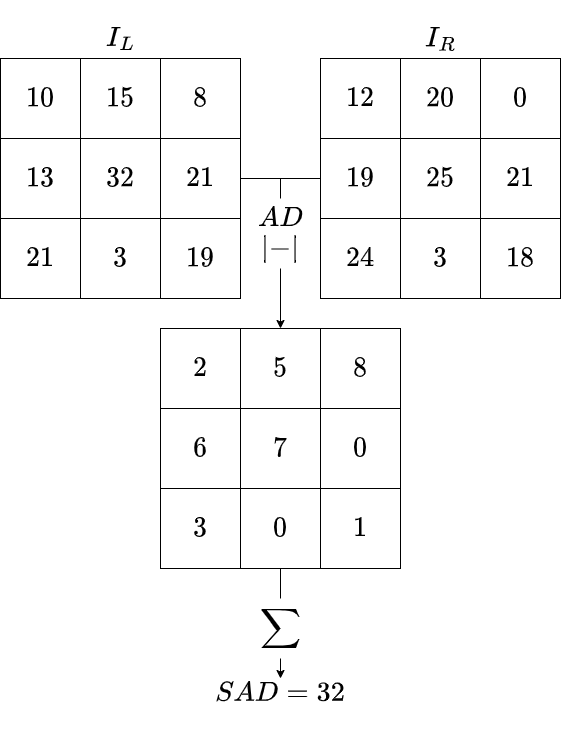
\includegraphics[width=0.5\linewidth]{Images/Chap_4/SAD.png}
    \caption{Diagram representing the $SAD$ cost function between two $3\times3$ patches. From \cite{malinowski_uncertainty_2024}}
    \label{fig:SAD}
\end{figure}

\subsection{Uncertainty Model for Epipolar Images Intensities}
To maintain simplicity in this section, we will not consider panchromatic images, such as Pléiades products, encoding the reflectance values as positive integer, usually contained in $[0, 5000]$. Instead, we consider grayscale images that have intensity levels quantified within the range $[0, 255]$, which will represent our measurable space $\X$.

\begin{remark}
    This hypothesis is not constraining as we can easily normalize reflectances in order to encode them using 8-bit integers value, although doing so reduces the precision of the initial images. Moreover, this normalization step is often required to fit a given format, for instance if the images must be processed by a CNN trained on 8-bit integers.
\end{remark}

We hypothesize that a pixel's intensity value can deviate around its its observed value with a range of $\pm i_\sigma$, with the observed value being the most likely. This specific hypothesis as it remains simple and relatively plausible with regards to the processing leading to the epipolar images. We suppose that the uncertainty from the noise of the sensor capturing the image, from pre-processing steps such as atmospheric correction or epipolar resampling (see section \ref{sec:uncertainty_cars}) or from the quantification of observed radiometric values into integers, are not exactly known, but can be model by a possibility distribution. This hypothesis does not seem far-stretched depending on the range of possible intensities. Consequently, we model the uncertainty of each pixel $p\in I_L,I_R$ intensity with a possibility distribution $\pi$, centered around the observed intensity $i_p\in[0,255]$:
\begin{equation}
    \pi(i_p)=1,\quad \pi(i_p\pm i_\sigma)=\alpha\,,
\end{equation}\label{eq:pixel_possibility}
with $\alpha \in [0,1]$. The $\pm$ indicates that both positive and negative values are considered. To remain simple, we chose $i_\sigma=1$ in the following, which is relatively narrow but simplifies without impacting our reasoning. In our simulation, $\alpha = 0.3$ for pixels in the left image and $\alpha = 0.4$ for pixels in the right image\commanue{Je ne sais pas si tu synthétises les valeurs quelque part mais ce serait cool, ça peut être un tableau en annexe, sinon ça oblige à relire la section pour retrouver les valeurs}. We use different values of $\alpha$ for the left and right images because the uncertainty model may vary between images due to differences in exposure, noise levels, or camera calibration. The values on themselves are chosen arbitrarily for the purpose of this example. From a credal set interpretation, this model effectively states that we accept any probability distribution supported within $[i_p - 1, i_p + 1]$ where the probability measure $P$ satisfies $\{P(A) \leq \sup_{i \in A} \pi(i)\}$ as an acceptable model for our uncertainty. The mass distribution function $m_p$ associated to this credal set possesses two focal sets $a^p$:
\begin{eqnarray}
    &m_p(a^p_1=\opi i_p, i_p\cli)=1-\alpha\,\nonumber\\
    &m_p(a^p_2=\opi i_p-1, i_p + 1\cli)=\alpha\,\label{eq:pixel_mass}
\end{eqnarray}
with $\opi\cdot, \cdot\cli$ referring to integer intervals. In particular, $\opi i_p, i_p\cli$ correspond to the singleton $\{i_p\}$.

\begin{remark}
    The hypothesis of modelling the uncertainty on image intensities by possibility distributions does not consider uncertainty from potentially bigger sources of errors, such as satellite vibrations during the acquisition, or errors in the computations of epipolar lines. Those type of errors have been encountered on some Pléiades acquisitions, and lead to significant biases and errors on the final DSM, that our simple model does not account for. However, the CO3D mission will acquire images using a CCD matrix sensor and not a push-broom sensor as used in Pléiades, so we can safely assume that those problems should not be encountered on images from the CO3D mission.
\end{remark}

\subsection{Dependency Model between Epipolar Images}
We presented the uncertainty models for pixels in both images, but we also need to define the dependency model between every pixel of both images. Indeed, as some pixels between images represent the light reflected by the same object, it seems natural that their (uncertain) values are correlated. In our case, we propose to model their dependency with the product copula if the pixels are not from the same physical object, meaning that the value of their intensities are independent. For pixels belonging to the same object, we model their dependency by a Gaussian copula with a covariance matrix $R$. Those copulas were presented in equation \eqref{eq:gaussian_copula} from chapter \ref{chap:representation_of_uncertainty}. The correlation values inside the covariance matrix are based on a segmentation $S:(I_L\cup I_R)\rightarrow\opi1,K\cli$, $K\in\mathbb{N}$, of the images. This segmentation is the result of a \textit{k-means} clustering performed on the ground truth disparity map. Example of such a clustering is presented in figure \ref{fig:clustering_example}, with $K=8$. Given the segmentation $S$ and two pixels $(p, q)\in(I_L\cup I_R)^2$, their covariance is determined by
\begin{equation}
    \sigma(p, q) =
    \begin{cases}
        1 &\text{ if }p=q,\\
        \rho_K, &\text{ if } p\ne q\text{ and }S(p)=S(q)\,, \\
        0 & \text{otherwise}\,.
    \end{cases}\label{eq:correlation}
\end{equation}
where $0<\rho_k<1$ is the correlation of pixels belong to segment $k\in\opi 1, N\cli$. Given a set of pixels $\{p_1, \dots, p_n\}\subseteq(I_L\cup I_R)^2$, their covariance matrix $R$ is therefore:
\begin{align}
    R = \begin{bmatrix}
            1 & \sigma(p_{1}, p_{2}) & \dots & \sigma(p_{1}, p_{n-1}) & \sigma(p_{1}, p_{n})\\
            \sigma(p_{2}, p_{1}) & 1 & \dots & \sigma(p_{2}, p_{n-1}) & \sigma(p_{2}, p_{n})\\
            \dots & \dots & \dots & \dots & \dots\\
            \sigma(p_{n-1}, p_{1}) & \sigma(p_{n-1}, p_{2}) & \dots & 1 & \sigma(p_{n-1}, p_{n})\\
            sigma(p_{n}, p_{1}) & \sigma(p_{n}, p_{2}) & \dots & \sigma(p_{n}, p_{n-1}) & 1
        \end{bmatrix}
\end{align}

In practice, we will only compute the correlation matrix between the two windows from the reference and secondary images that are compared. The windows have a $3\times 3$ shape, we thus consider Gaussian $18-$copulas to model the dependency between pixels. This copula will be used for joining marginal masses in the uncertainty propagation step using equation \eqref{eq:joint_mass} from the previous chapter. It will also be used to sample noise for Monte Carlo sampling in section \ref{sec:montecarlo}.

\begin{remark}
    Gaussian copulas are a popular and simple model to represent dependency between more than $2$ variables. The different $2$-copulas presented in section \ref{sec:copulas} cannot always be defined in more than $2$ dimensions. Another method for modelling the dependency for more than $2$ variables is to express a $n$-copula as a combination of $2$-copulas, which is called a vine copula (\cite{czado_vine_2022}). However this is a complex subject that is not adapted to our type of dependency, and is therefore not explored in this thesis.
\end{remark}

\begin{figure}
    \centering
    \begin{subfigure}[t]{0.5\linewidth}
        \centering
        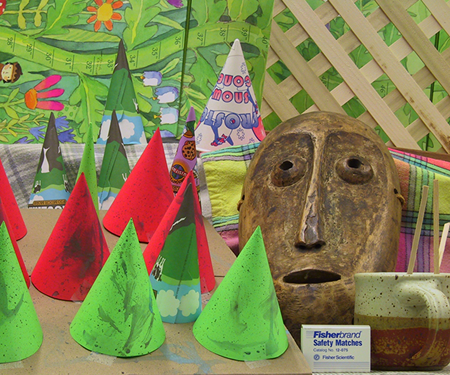
\includegraphics[width=0.9\linewidth]{Images/Chap_4/im2.png}
        \caption{Colored left image}
        \label{fig:color_cones_image}
    \end{subfigure}\hfill
    \begin{subfigure}[t]{0.5\linewidth}
        \centering
        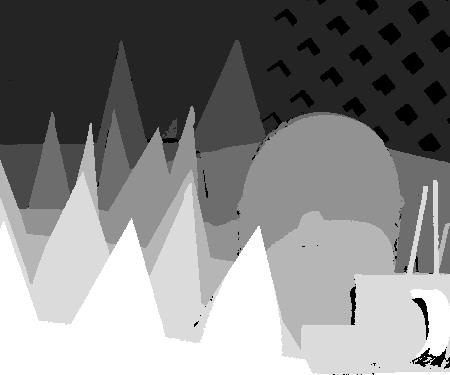
\includegraphics[width=0.9\linewidth]{Images/Chap_4/cluster.jpg}
        \caption{Proposed clustering of the image (\textit{k-means} with $k=8$)}
        \label{fig:cluster}
    \end{subfigure}
    \caption{Middlebury 2003 Cones left image, and a clustering computed from the disparity ground truth.}
    \label{fig:clustering_example}
\end{figure}

During our simulations, the segmentation contains $K=8$ different clusters. For every $k$ in $\opi1,K\cli$, $\rho_k$ is assigned an value between $0.9$ and $1$ in order to really emphasize on their correlation.

\begin{remark}
    The segmentation is based on the ground truth disparity map. This means that two objects with similar disparities located at opposite sides of the image will be considered as belonging to the same object and thus correlated. In practice, those pixels are never compared as we only measure the dissimilarity between small windows in a restricted disparity range. The clustering is thus only considered at a \textit{local} scale. 
    
    Secondly, the segmentation allows to compute the Gaussian copula, which will be used to propagate the uncertainty models. We will validate the uncertainty propagation in section \ref{sec:montecarlo} with Monte Carlo samples using the same copula. As long as the copulas used are the same between the propagation and validation, it does not really matter which correlation matrix is used. We still tried to create a realistic but simple model for the sake of the example, but it is not requirement from a theoretical point of view.
\end{remark}

\section{Propagating the Uncertainty with Belief Functions and a Copula}
Having defined both marginal models for pixel intensities using possibility distributions as well as dependency models using copulas, we can know join them all to construct a multivariate uncertainty model. As seen in section \ref{subsec:necessity_functions}, the multivariate model is a belief function and not necessarily a possibility distribution. We will see in this section that the multivariate belief function can then be used to compute the uncertainty regarding the cost curve. 

\subsection{From Multivariate Uncertainty Models to the Propagated Model}
We first detail how multivariate models are used to propagate uncertainty in the precise case. We will then do the same in the imprecise setting by analogy.

Consider a mapping $f:\X_1\times\X_2\rightarrow\mathcal{Z}$ from a product space $\X_1\times\X_2$ to a space $\mathcal{Z}$, which propagates multiple random variables $X_1$, $X_2$ to a new random variable $Z=f(X_1, ~X_2)$. In our case, $f$ will be the SAD cost function propagating the intensities to the matching cost. When considering precise probabilities, the probability of $Z=z$ is obtained by summing the probabilities of all events $X_1=x_1$, $X_2=x_2$ whose image by $f$ is $z$: 
\begin{align}\label{eq:precise_propagate_proba}
    \forall z\in\mathcal{Z}, P_Z(z)=\sum_{\substack{x_1,x_2\\z=f(x_1,x_2)}}P(x_1,x_2).
\end{align}
where $P(x_1,x_2)$ is the joint probability, which is linked to its marginals by a copula $C$. $P_Z$ only needs to be evaluated for every combination of atoms of $\X_1$ and $\X_2$.

\begin{example}
    Consider the same setting as example \ref{ex:copulas}, where a dealer throws two coins in a separate room. The coins seem fair when looked at independently. In this example, a coin landing on heads rewards you with $1$€(or any currency of your choice), and a coin landing on tails rewards you with $0$€. So you earn $2$€ if both coins land on heads, $1$€ if only one coin land on heads and the other on tails, and $0$€ if both coins land on tails. We are interesting in the uncertainty regarding you earnings, noted $Z$.
    
    In example \ref{ex:copulas}, we consider $3$ different cases, each leading to a different copula $C$ modelling the dependency between the probability $P_1$ of first coin and $P_2$ of the second coin. For each copula, we then computed the joint probability $P$.
    
    In the first case, where coin throws were independent, we saw that the joint probability $P$ was:\\
    \begin{minipage}[b]{0.5\linewidth}
    \begin{align*}
        & P(\text{heads}, ~\text{heads}) = 0.25\\
        & P(\text{heads}, ~\text{tails}) = 0.25
    \end{align*}
    \end{minipage}
    \begin{minipage}[b]{0.5\linewidth}
    \begin{align*}
        & P(\text{tails}, ~\text{tails}) = 0.25 \\
        & P(\text{tails}, ~\text{heads}) = 0.25
    \end{align*}
    \end{minipage}
    In that case, it holds that the probability $P_Z$ of our earnings are:
    \begin{align*}
        & P_Z(Z=2) = P(\text{heads}, ~\text{heads}) = 0.25\\
        & P_Z(Z=1) = P(\text{heads}, ~\text{tails}) + P(\text{tails}, ~\text{heads}) = 0.5 \\
        & P_Z(Z=0) = P(\text{tails}, ~\text{tails}) = 0.25
    \end{align*}
    
    In the second case, where coin throws were rigged to land on the same side, we saw that the joint probability $P$ was:\\
    \noindent
    \begin{minipage}[b]{0.5\linewidth}
    \begin{align*}
        & P(\text{heads}, ~\text{heads}) = 0.5\\
        & P(\text{heads}, ~\text{tails}) = 0
    \end{align*}
    \end{minipage}
    \begin{minipage}[b]{0.5\linewidth}
    \begin{align*}
        & P(\text{tails}, ~\text{tails}) = 0.5\\
        & P(\text{tails}, ~\text{heads}) = 0 
    \end{align*}
    \end{minipage}
    Following the same methodology, we have:\\
    \noindent\begin{minipage}[b]{0.33\linewidth}
    \begin{align*}
        & P_Z(Z=2) = 0.5
    \end{align*}
    \end{minipage}
    \begin{minipage}[b]{0.33\linewidth}
    \begin{align*}
        & P_Z(Z=1) = 0
    \end{align*}
    \end{minipage}
    \begin{minipage}[b]{0.33\linewidth}
    \begin{align*}
        & P_Z(Z=0) = 0.5
    \end{align*}
    \end{minipage}
    
    In the third case, where coin throws were rigged to land on opposite sides, we saw that the joint probability $P$ was:\\
    \noindent\begin{minipage}[b]{0.5\linewidth}
    \begin{align*}
        & P(\text{heads}, ~\text{heads}) = 0\\
        & P(\text{heads}, ~\text{tails}) = 0.5
    \end{align*}
    \end{minipage}
    \begin{minipage}[b]{0.5\linewidth}
    \begin{align*}
        & P(\text{tails}, ~\text{tails}) = 0\\
        & P(\text{tails}, ~\text{heads}) = 0.5
    \end{align*}
    \end{minipage}
    Therefore:\\
    \begin{minipage}[b]{0.33\linewidth}
    \begin{align*}
        & P_Z(Z=2) = 0
    \end{align*}
    \end{minipage}
    \begin{minipage}[b]{0.33\linewidth}
    \begin{align*}
        & P_Z(Z=1) = 1
    \end{align*}
    \end{minipage}
    \begin{minipage}[b]{0.33\linewidth}
    \begin{align*}
        & P_Z(Z=0) = 0
    \end{align*}
    \end{minipage}
\end{example}

Determining every $(x_1, x_2)$, whose image by $f$ equals $z$, is not always trivial. This becomes even more complex when considering $n>2$ marginal variables. Similarly, the joint probability $P(x_1,x_2)$ is computed using a H-volume, which is the sum of $2^n$ terms, thus also increasing exponentially with the dimension.

There are multiple ways of extending equation \eqref{eq:precise_propagate_proba} to the imprecise setting, as there are multiple ways of aggregating imprecise models using a copula. We presented in chapter \ref{chap:joining_credal_sets} three methods for joining marginal credal sets, creating three different multivariate credal sets $\M_{robust}$, $\M_{mass}$ and $\M_{agg}$.

The robust approach of extending equation \eqref{eq:precise_propagate_proba} is based on the robust approach from section \ref{sec:robust_method}. Given $n$ marginal credal sets $\M_i$, we can join them using a copula $C$ into a credal set $\M_{robust}$ as in \eqref{eq:robust_set}. The propagated uncertain model $\M^Z_{robust}$ is then defined as:
\begin{align}
    \M^Z_{robust} = \{P_Z~|~\forall z\in Z, P(z)=\sum_{\substack{x_1,\dots,x_n\\z=f(x_1,\dots,x_n)}}P(x_1,\dots,x_n), ~P\in\M_{robust}\}
\end{align}
Practically, it consists in sampling every probability $P_i$ from each marginal credal set $\M_i$ and joining them using Sklar's theorem \ref{theorem:sklar} into a multivariate probability $P$. Then for each $z=P(x_1,\dots,x_n)$, we can compute $P_Z$ from $P$ using \eqref{eq:precise_propagate_proba}. In short, each sample $(P_1,\dots,P_n)$ leads to a new $P$, itself leading to a new $P_Z$. Sampling through every $(P_1,\dots,P_n)$ thus leads to the estimation of the uncertain model of $Z$. This method is complicated to compute, but correctly propagates uncertainty.

We saw that it was easier to compute $\M_{mass}$ than $\M_{robust}$. Another way of approximating the uncertainty model of $Z$ is to compute it using $\M_{mass}$. This is done by replacing the probability on atoms from equation \eqref{eq:precise_propagate_proba} with the joint mass $m_\times$ from equation \eqref{eq:joint_mass} \cite{gray_dependent_2021}. Consider $n$ uncertain variables $X_i$, each modeled by a mass distribution function $m_i$ with focal sets $(a^i_j)$. Given their multivariate mass $m_\times$, it is possible to compute the mass distribution function $m_Z$ of a random set $Z=f(X_1,\dots,X_n)$ as:
\begin{align}
    \forall a^Z\subseteq\mathcal{Z}, m_Z(a^Z) = \sum_{\substack{a^1_i, \dots, a^n_j\\a^Z=f(a^n_1,\dots, a^n_j)}}m_\times(a^1_i, \dots, a^n_j)\label{eq:mass_propagated}
\end{align}

In order to compute the propagated mass $m_Z$ (and its associated belief function) from equation \eqref{eq:mass_propagated}, two difficulties arise. The first one is to determine what the focal sets $a_Z$ of $m_Z$ will be, which corresponds to the subscript $a^Z=f(a^n_1,\dots, a^n_j)$ of the sum. Computing the image of $f$ for every combination of focal sets $(a^1_i, \dots, a^n_j)$ is even more difficult than in the precise case, as we are computing images of sets instead of real numbers. The second difficulty is to compute the joint mass $m_\times$, as in the case of the SAD it requires to compute the $H$ volume of an $18$-copula. Those difficulties will be addressed in the following sections \ref{sec:propagated_focal_sets} and \ref{sec:propagated_masses}

We saw in chapter \ref{chap:joining_credal_sets} that in the situation where marginals are possibility distributions, $\M_{mass}$ and $\M_{agg}$ have the same bounds on Cartesian products of events (see equation \eqref{eq:inclusion_necessity}). We will thus only compute the lower bounds $Bel_\times$ of $\M_{mass}$ as it directly provides the bounds of $\M_{agg}$ on those events.

\subsection{Computing the Propagated Focal Sets}\label{sec:propagated_focal_sets}
In this section, we will detail how we compute the SAD image of marginal focal sets. Computing the image of sets needs to be treated with caution in the general case. However in our case, because we chose marginal focal sets with a simple form, and because we are using a relatively regular cost function, computing the image does not raise any significant problem.

Given a pixel $p$, we consider the mass distribution $m_p$ of equation \eqref{eq:pixel_mass} and its two focal sets $a_1^p$ and $a_2^p$. For every pair of pixels $p\in I_L, q\in I_R$, we note $\AD_{pq}=|i_p - i_q|$, where $i$ refers to a pixel's intensity. Given $m_p$, There exist $3$ focal sets related to the absolute difference:
\begin{itemize}
    \item $a^{\AD}_1$ is the image of the AD of $a^p_1$ and $a^q_1$
    \item $a^{\AD}_2$ is the image of the AD of $a^p_2$ and $a^q_1$ or $a^p_1$ and $a^q_2$
    \item  $a^{\AD}_3$ is the image of the AD of $a^p_2$ and $a^q_2$
\end{itemize}
The non-monotonicity of the absolute value around $0$ needs to be taken into account to compute their exact image through the AD. Indeed, if a value $x$ is in $[-1,1]$, then its absolute value will be in $[0,1]$. Applying this remark to the AD yields the following focal sets:
\begin{align*}
    a^{\AD}_1&=\opi\AD_{pq},~\AD_{pq}\cli\,,\\
    a^{\AD}_2&=\opi\max(0, \AD_{pq} - 1),~\AD_{pq} + 1\cli\,,\\
    a^{\AD}_3&=\opi\max(0, \AD_{pq} - 2),~\AD_{pq} + 2\cli\,,
\end{align*}

Focal sets of the final SAD are then computed by simply summing the bounds of the $9$ AD focal sets (as in figure \ref{fig:SAD}), for every combination of those focal sets. 

\begin{remark}
    In many cases, different combinations of $\AD$ focal sets will lead to the same $\SAD$ focal set. Actually, if every $\AD$ is greater than $2$ (so that each $a^\AD_i$ is symmetric with regard to its $\AD$) there will only be $19$ focal sets $a^\SAD$ for the $\SAD$, and they are of the following form:
    \begin{align*}
        a^\SAD = \opi\SAD-t,\SAD+t\cli,\text{ with }t\in\opi0, ~18\cli
    \end{align*}
    In comparison, there are $3^9=19683$ different combinations of $\AD$ focal sets.
\end{remark}

\subsection{Computing the Mass of Propagated Focal Sets}\label{sec:propagated_masses}
%\section{Leveraging Specificities to Accelerate Computations}
Now that the bounds of the $\SAD$ have been computed, we need to compute the associated mass. Computing the joint mass over two $3 \times 3$ windows is however significantly more complex. For each combination of marginal focal sets, the joint mass $m_{\times}$ is computed using the $H$-volume of an $18$-copula, involving a sum of $2^{18}$ terms. Given that the uncertainty for each pixel is represented by $2$ focal sets, we need to evaluate $2^{18}$ combinations of these focal sets in total. This computation can thus become quite costly in memory and computation time, especially when computing it over a whole image.

A strategy to reduce computation time is to leverage the fact that focal sets derived from a possibility distribution (or equivalently from its necessity measure) form a nested family of sets. As a reminded, a nested family of sets is a family $a_1\subset\dots\subset a_n$ of sets. We saw that in that case,
\todoroman{Dire que pour le cas où AD>2, $Bel_Z$ est encore une mesure de nécessité. On pourrait donc calculer son $\pi$. On sait donc qu'elle est déterminée par les $37$ valeurs de $\Pi$ sur chaque atome. Faire une digression qui dit dans quel cas on à ce comportement là ?
Et sinon: dans tous les cas on peut faire $Bel=C(Nec_1,...,Nec_n)$ et donc calculer rapidement Bel sur les évennements qui nous intéressent sans passer par m ou le H volume.}
For simplicity, the following observations will be detailed in the case where there are $n=2$ sources of uncertainty to join, but they hold for every $n\geqslant2$\commanue{Mayday, encart pour signaler une digression ou disons une explication qui sort du cas de base !}. Propagating two necessity measures\commanue{c'est toujours perturbant pour moi , je ne sais pas faut pas être trop répétitif mais juste rappeler que considère la necessity function définie par la possibility distribution. Je sais que c'est évident pour un matheux mais le truc c'est que le manuscrit s'adresse un peu à tout le monde} $\mathrm{Nec}_1:2^{\X_1} \rightarrow [0,1]$ and $\mathrm{Nec}_2: 2^{\X_2} \rightarrow [0,1]$ through a mapping $f: \X_1 \times \X_2 \rightarrow \mathcal{Z}$ using a copula $C$ does not generally result in a necessity measure, but rather a belief function.

For the special case where\commanue{c'est le cas spécial de la démonstration en dimension 2 qui correspond à notre pb à plus de 2 dimension, non parce que là je suis perdue}:
\begin{itemize}
    \item $\mathrm{Nec}_1$ and $\mathrm{Nec}_2$ are defined by symmetric uni-modal possibility distributions (typically triangular possibilities)
    \item $f$ is a monotone function applied to a linear combination $\alpha X_1 + \beta X_2 + \gamma$, with $(\alpha, \beta, \gamma) \in \mathbb{R}^3$
\end{itemize}
then the focal sets of $\mathrm{Nec}_{X_1}$\commanue{pourquoi c'est $x_1$ l'indice  et pas juste 1 ?} and $\mathrm{Nec}_{X_2}$ are families of nested sets that can be represented as\commanue{je comprends pas tu as deux intervalles qui se promènent tous seuls sur une ligne ! Juste pour moi, ça sort d'où ? C'est évident tout le monde le sait ? C'est par définition ? ça se démontre ?}:
\begin{align*}
    [\overline{X}_1-\delta x^1_i, \overline{X}_1+\delta x^1_i]\quad[\overline{X}_2-\delta x^2_j, \overline{X}_2+\delta x^2_j]
\end{align*}
with $\overline{X}_1\in\X_1,~\overline{X}_2\in\X_2$ and $\delta x^1_i,~\delta x^2_j$ positive scalars. This results in the focal sets $a_{ij}$ of $Z = f(X_1, X_2)$ having the following expression\commanue{pareil c'est censé être straightforward comme résultat ?}:
\begin{align*}
    a_{ij} = \left[ \alpha \overline{X_1} + \beta \overline{X_2} + \gamma - (|\alpha| \Delta x^1_i + |\beta| \Delta x^2_j), \right. \\
                 \left. \alpha \overline{X_1} + \beta \overline{X_2} + \gamma + (|\alpha| \Delta x^1_i + |\beta| \Delta x^2_j) \right],\commanue{pourquoi c'est $\Delta$ et plus $\delta$ ?}
\end{align*}
Those focal sets form a nested family of sets, which is a characteristic of necessity measures \cite{shafer_mathematical_1976}\commanue{Je comprends pas l'enchainement de la remarque on vient de le dire que c'était nested donc je ne suis plus là. C'est un nouveau élément que tu ajoutes ?}. When a monotone function is applied to these focal sets, the nesting property is maintained, although the symmetry of the sets might be lost\commanue{comme je comprends pas, question surement bête mais donc tu n'as pas encore utilisé que f était monotone. Donc peut-être définir d'abord f et ensuite faire remarquer qu'elle est monotone.Je veux bien accepté certains résultats de maths car je ne suis pas à l'aise avec les notions. Mais là dans ta démonstration j'ai quand même l'impression d'avoir les éléments pas dans l'ordre logique pour suivre le raisonnement. Donc soit j'ai vraiment rien compris et dans ce cas laisse tomber mon commentaire soit remet un peut d'ordre dans la manière avec laquelle tu avances les arguments les un après les autres}. This implies that $\mathrm{Bel}_Z$ (the belief function derived from $Z$) behaves as a necessity measure under these conditions.

On the other hand, for more sophisticated functions, such as multiplication, exponential functions, or sigmoid functions, the nesting property might not hold. It's often easy to find counterexamples where the nested nature of the focal sets is disrupted when such functions are applied. The upcoming example illustrates this situation\commanue{tu fais des encarts pour metter en lumière des contres exemples mais tu mets pas en lumière les éléments utiles à ta démonstration.}.

\begin{example}\commanue{je ne sais pas si cette digression est vraiment utile. J'ai un peu le sentiment de faire les poupées russes ou de sauter du coq à l'âne ça dépend des moments dans la démonstration. Je t'avoue qu'ici je ne sais plus dire ce que tu as démontré ou non et où on en est clairement de pb posé en début de chapitre.}
    Consider the function $f(x_1,x_2)=(x_1^2+1)+(x_2^2+1)$, and the following marginal mass functions $m_1$ and $m_2$:
\begin{align*}
    &m_{1}([0]) = m^{1}_1>0,\, &m_{2}([1]) = m^{2}_1>0\,,\\
    &m_{1}([-2,2]) = m^{1}_2>0,\, &m_{2}([0,2]) = m^{2}_2>0\,.
\end{align*}
After propagating through the function $f$ with a copula $C$, one gets the joint mass $m_\times$:
\begin{eqnarray*}
    m_\times(f([0],[1])) =& m_\times([3]) &= C(m^{X_1}_1,m^{X_2}_1)\,,\\
    m_\times(f([-2,2],[1])) =& m_\times([3,7]) &= m^{X_2}_1 - C(m^{X_1}_1,m^{X_2}_1)\,,\\
    m_\times(f([0],[0,2])) =& m_\times([2,6]) &= m^{X_1}_1 - C(m^{X_1}_1,m^{X_2}_1)\,,\\
    m_\times(f([-2,2],[0,2])) =& m_\times([2,10]) &= 1 - m^{X_1}_1 - m^{X_2}_1 + C(m^{X_1}_1,m^{X_2}_1)\,.
\end{eqnarray*}
For most copulas and mass functions (for instance $C=C_\Pi$, and $m^1_1=m^1_2=m^2_1=m^2_2=m^1_1=0.5$), the output focal sets of $m_\times$ do not form a nested family, and thus defines a belief function that is not a necessity function.
\end{example}

The nesting property for uni-modal symmetric possibilities and monotone functions can be leveraged to streamline the computation of the bounds and masses of focal sets, particularly when all (AD) exceed $2$\commanue{Donc Manue perdue demande où on en est. Il faudrait une phrase avec un statut clair de ce que tu as démontré et comment tu repares sur ton pb. Là honnêtemnt je ne sais pas quoi faire avec cette remarque.}. This condition helps to circumvent the complications arising from the non-monotonic behavior of the absolute value function near $0$\commanue{je sais pas c'est un peu abrupte les enchainements donc si je comprends un peu, c'est par raport au fait que AD n'est pas monotone et que ça change en 0. Oui mais là honnêtement il te manque des bouts}.

In the scenario where the focal sets are nested\commanue{c'est quoi l'univers parallèle dans lequel c'ets pas nested ? C'est quoi le lien avec avant ? Visiblement dans la suite on est encore en dimension 2 donc c'est fini a priori}, we can use equation \eqref{eq:sklar_on_necessity} to compute the belief of any focal sets $a^1_i$ and $a^2_j$ associated with the necessity functions $\mathrm{Nec}_1$ and $\mathrm{Nec}_2$ respectively. For any copula $C$ it holds that:
\begin{align*}
    \mathrm{Bel}_\times(a^1_i, a^2_j) = C(\mathrm{Nec}_1(a^1_i),~\mathrm{Nec}_2(a^2_j))
\end{align*}

This implies that the joint belief function $\mathrm{Bel}_\times$ can be efficiently derived using only the marginal necessity functions $\mathrm{Nec}_X$ and $\mathrm{Nec}_Y$ along with the copula. Consequently, there is no requirement to calculate the joint mass directly, thereby eliminating the need to evaluate the $H$-volume as described by equation \eqref{eq:hvolume}. This means that the belief of every cylindrical event\commanue{et notre pb c'est cylindrique ou pas ? C'est assez perturbant comme démonstration car on a un problème mais on raisonne sur autre chose et on fait des remarques générales qui s'appliquent ou non et vu mon niveau je sais pas le dire. Les passages théoriques dans ce chapitre sont assez déroutants.} can be computed easily, with a single evaluation of a copula (contrary to what is required when using the H-volume). Computing the plausibility $\mathrm{Pl}_\times$ of cylindrical events $A_1\times A_2\subseteq\X_1\times\X_2$ is also straightforward by noticing that:
\begin{align*}
    \mathrm{Pl}_\times(A_1\times A_2) =& 1-\mathrm{Bel}_\times\left((A_1\times A_2)^c\right)\\
    =& 1 - \sum_{a_1\times a_2\subseteq(A_1\times A_2)^c}m_\times(a_1,a_2)\\
    =& 1 - (~\sum_{a_1\times a_2\subseteq A_1^c\times \X_2}m_\times(a_1,a_2) + \sum_{a_1\times a_2\subseteq \X_1\times A_2^c}m_\times(a_1,a_2) \\
    &- \sum_{a_1\times a_2\subseteq A_1^c\times A_2^c}m_\times(a_1,a_2) ~)\\
    =& 1 - \mathrm{Bel}_1(A_1^c) - \mathrm{Bel}_2(A_2^c) + \mathrm{Bel}_\times(A_1^c\times A_2^c)
\end{align*}
For events that are not cylindrical, then we need to compute the joint mass, either with the H-volume or using the fact that (\cite{shafer_mathematical_1976})\commanue{encore une fois le rapport avec le problème de base. Après si tu discuter plus sur la théorie et ensuite l'appliquer à ton cas particulier j'ai pas de souci mais faut pas l'organiser comme cela. Là tu es parti de l'application et tu théorises au milieu.}:
\begin{align}
    \forall A\subseteq\X,~m_\times(A)=\sum_{a\subseteq A}(-1)^{|A/a|}\mathrm{Bel}_\times(A)\label{eq:bel_to_mass}
\end{align}

Another issue arises when computing the joint belief $\mathrm{Bel}_\times$ is that evaluating the copula for a high number of variables can become computationally heavy. This is the case for copulas for which only a closed form of its density is known, such as the family of Gaussian copulas. In that case, each evaluation necessitates integrating an $n$-variate function, leading to significant computational expense\commanue{clairement cette remarque c'est comme si tu n'avais jamais mentionné l'application de départ.}.

In our experiments\commanue{on revient sur l'application, mais alors j'ai rien compris car on a démontré quoi, comment ça s'applique dans notre cas et qu'est ce qu'on gagne. Une petite phrase de synthèse ne serait pas du luxe.}, we processed images of size $375 \times 450$ with a disparity range of $[-60, 0]$\commanue{soit tu dis après avoir décris le pipeline que tu utlises les images middlebury mais là donner la taille alors qu'on saura que c'est middlebury plus tard c'est bizarre}. This resulted in the computation of over $10^7$ belief functions. Each belief function integrates the uncertainty from $2 \times 3 \times 3 = 18$ pixels, each having $2$ distinct focal sets. Consequently, we must compute the integral of more than $10^7 \times 2 ^{18}$ $18$-variate functions if we want to completely determine $\mathrm{Bel}_\times$, which is extremely time-consuming, even with optimized parallel processing. In practice, the number of evaluations is smaller as some combinations of marginal focal sets lead to the same propagated focal set. Nevertheless, calculating an $18$-dimensional Gaussian copula takes approximately $20$ seconds on an AMD EPYC $7713$ $64$-Core Processor at $2$ GHz, using Python and the SciPy library. However, we can significantly reduce the computation time by exploiting specific properties of our models and the copula\commanue{attends à quoi servait les premiers paragraphes dans cette section. J'avoue que je n'arrive plus à savoir ce qu'on a déjà démontré, ce que peut utiliser, ce qu'il manque}.

Indeed\commanue{On peut pas commencer un paragraphe avec indeed, c'est contraire à ma religion. Là c'est clairement lié à ce qui précède}, if the variables can be divided into multiple mutually independent sets of variables, the evaluation of the copula or of the H-volume is reduced\commanue{c'est quoi le lien entre avec le pb ? En fait on dirait le retour du sort apparition de proposition mais sans les encarts, c'est la version furtive du sort.}. For instance\commanue{là l'objectif c'est de démontrer la propriété précédente mais de manière générique}, suppose that we can split the $n$ variables into two mutually independent sets $\{X_1,\dots,X_k\}$ and $\{X_{k+1},\dots,X_n\}$ with $k\in\opi1,n-1\cli$. Let $F_1,\dots, F_n$ be their marginals CDF. Then it holds that there exists a $k$-copula $C'$ and a $(n-k)$-copula $C''$ such that:
\begin{align*}
    &\forall (x_1,\dots,x_n)\in\X_1\tdt\X_n,\\
    &C(F_1(x_1),\dots,F_n(x_n))=C'(F_1(x_1),\dots, F_k(x_k))\cdot C''(F_{k+1}(x_{k+1}),\dots,F_n(x_n))
\end{align*}
which uses the same composition as vine copulas \cite{czado_vine_2022}, where the pair copula is the product copula. Knowing other types of dependency would allow to express the $n$-copula in terms of multiple lower dimension copulas, but the nature of our problem do not permit us to know such dependencies\commanue{j'ai craqué en lisant cette phrase parce que j'ai l'impression que j'ai fini par perdre de vue la nature de problème de mon côté}. 

\begin{remark}
    If a $n$-copula $C$ can be expressed as the product of a $k$-copula $C'$ and a $(n-k)$-copula $C''$, then the H-volume of $C$ is the product of the H-volume of $H'$ of $C'$ and the H-volume $H''$ of $C''$. Indeed, for all $(u_1\tdt u_n)\in[0,1]^n$ and for all $(v_1\tdt v_n)\in[0,1]^n$ such that $\forall i\in\opi1,n\cli, u_i\leqslant v_i$, it holds that:
    \begin{align*}
        {H'}_{u_1,\dots, u_k}^{v_1,\dots, v_k}\times {H''}_{u_{k+1},\dots, u_n}^{v_{k+1},\dots, v_n} =& \left(\sum_{w_i\in\Pi_{i=1}^{k}\{u_i,v_i\}}(-1)^{|\{w_i~|~w_i=u_i\}|}C'(w_1,\dots,w_k)\right)\\
        &\times\left(\sum_{w_j\in\Pi_{j=k+1}^{n}\{u_j,v_j\}}(-1)^{|\{w_j~|~w_j=u_j\}|}C''(w_{k+1},\dots,w_n)\right)\\
        =& \sum_{w_i\in\Pi_{i=1}^{k}\{u_i,v_i\}}\times\sum_{w_j\in\Pi_{j=k+1}^{n}\{u_j,v_j\}}(-1)^{|\{w_i~|~w_i=u_i,~i\leqslant k\}|}\\
        &\times(-1)^{|\{w_j~|~w_j=u_j,~ j>k\}|}C'(w_1,\dots,w_k)C''(w_{k+1},\dots,w_n)\\
        =&\sum_{w_i\in\Pi_{i=1}^{n}\{u_i,v_i\}}(-1)^{|\{w_i~|~w_i=u_i\}|}C'(w_1,\dots,w_k)\\
        &\times C''(w_{k+1},\dots,w_n)\\
        =&H_{u_1,\dots, u_n}^{v_1,\dots, v_n}
    \end{align*}
\end{remark}

Extending this result to any number of independent subsets of $\{X_1, \dots, X_n\}$ is straightforward. This approach significantly simplifies the computation of the H-volume in high-dimensional spaces. Consider, for instance, splitting the set into two independent subsets: one containing $k$ elements and the other containing the remaining $n - k$ elements, with $k\in\opi1, n-1\cli$. Under this partitioning, the H-volume is now computed by evaluating a $k$-copula $2^k$ times, and a $n-k$ copula $2^{n-k}$ times instead of a $n$ copula $2^n$ times.
For comparison, splitting the aforementioned Gaussian $18$-copula into two Gaussian $9$-copula reduces the computation time from 20 seconds to approximately 1 second\commanue{ce qui est possible car les images sont indépendantes ??}. This demonstrates the substantial time savings achieved by decomposing the problem into smaller, independent parts.

Another\commanue{additional way ? en gros on peut cumuler les réductions, avec another c'est vague} way of reducing the computation time for Gaussian copulas is to notice that if its correlation matrix is of type:
\begin{equation}
    R=\begin{pmatrix}
        1 &  & \sigma & \dots & \sigma\\
         & & & & \vdots\\
        \sigma &  & 1 & & \sigma\\
        \vdots &  &  & & \\
        \sigma & \dots & \sigma &  & 1
    \end{pmatrix}\label{eq:corr_matrix_sym}
\end{equation}
with $\sigma\in[0,1]$, are\commanue{pb d'angalis, il est où le sujet?} exchange/permutation\commanue{ça veut dire quoi ?} symmetrical, \ie for every permutation $\sigma:\opi 1, n\cli\rightarrow\opi 1, n\cli$, and every $u_1,\dots,u_n\in[0,1]^n$\commanue{alors comme c'est entrecoupé de formule c'est pas simple à suivre}:
\begin{eqnarray*}
    C_R(u_1,\dots, u_n) = C_R(u_{\sigma(1)} ,\dots, u_{\sigma(n)})
\end{eqnarray*}
In our case, pixels of the same image and of the same object possess identical mass distribution functions, and their correlation matrix is similar to equation \eqref{eq:corr_matrix_sym}. Using this symmetry property allows to limit the number of necessary computation to determine either $\mathrm{Bel}_\times$ or $m_\times$ for those pixels. For instance, let consider a cluster of $k$ pixels with $2$ focal sets as in our simulations\commanue{c'est une autre digression ?}. Then only $k$ evaluations of the copula are necessary to determine every values of $m_\times$, instead of the previous $2^k$ evaluations\commanue{donc dans notre cas qu'on cherche à résoudre....}.\commanue{aloirs là clairement une conclusion car après toutes les digressions, les remarques, etc, je suis incapable de dire ce qu'on fait exactement et ce qu'on gagne}

\section{Envelopes Defined by Plausibility Levels}
To provide a concrete example of how to propagate uncertainty\commanue{étant donné que tu te places dans un cas particulier, je dirais jsute que tu appliques ton approach au images de middlebury, en plus tu as déjà dit que ton intervalle était de 60}, we utilized the \textit{Middlebury} dataset (\url{https://vision.middlebury.edu/stereo/data/scenes2003/}). This dataset includes pairs of left and right images along with their corresponding ground truth disparity maps. Figure \ref{fig:Cones} shows an example of such an image pair.
For each pixel in the left image, we calculated the SAD cost curve, incorporating the uncertainty model described in \eqref{eq:pixel_possibility}\commanue{en revanche l'approche utilisé pour faire le calcul est donnée en kit...}. The focal sets, representing the uncertainty associated with the SAD values at each considered disparity, are defined as intervals around the ``precise'' SAD value.

\begin{figure}[ht]
  \centering
  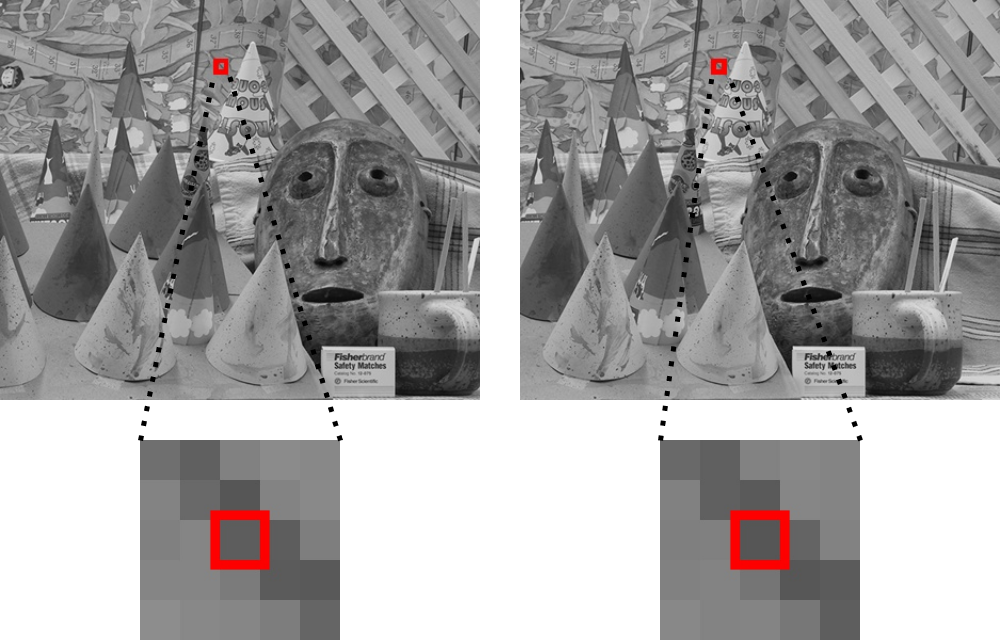
\includegraphics[width=0.8\linewidth]{Images/Chap_4/Cones.png}
  \caption{Homologous pixels in a pair of images. From \cite{malinowski_uncertainty_2024}}\label{fig:Cones}
\end{figure}

To visualize this uncertainty, we computed upper and lower envelopes for various plausibility levels $\gamma$\commanue{essayer de dire ce que représentent les différentes valeurs ou cets choisi au pif. J'ai sureemnt raté la conclusion précédente mais tu as parlé de Belx, tu as mentionné qqch par Pl mais c'était un peu noyé dans le reste. Donc on comprend ce que tu cherches à faire mais je défie quiconque pouvoir reproduire ce que tu as fait avec les indications que tu as donné}. These envelopes illustrate the largest (upper bound $\overline{a}$) and smallest (lower bound $\underline{a}$) focal sets where the plausibility, determined by Equation \eqref{eq:bel_pl}, meets or exceeds the given threshold $\gamma$: $\mathrm{Pl}(\overline{a}) \geqslant \gamma$. Consequently, there are two bounds for each level of $\gamma$.
At the plausibility threshold of 0 ($\mathrm{Pl}(\overline{a}) > 0$), the bounds represent the full support of the SAD values. Conversely, at a threshold of 1, the bounds converge to the values of the cost curve obtained in the ``precise'' setting (\ie, without accounting for uncertainty)\commanue{au temps pour moi un peu plus loin, j'ai ma réponse sur au moins deux valeurs pour gamma, les valeurs extrêmes.}.

\begin{figure}
    \centering
    \begin{subfigure}{0.48\linewidth}
        \centering
        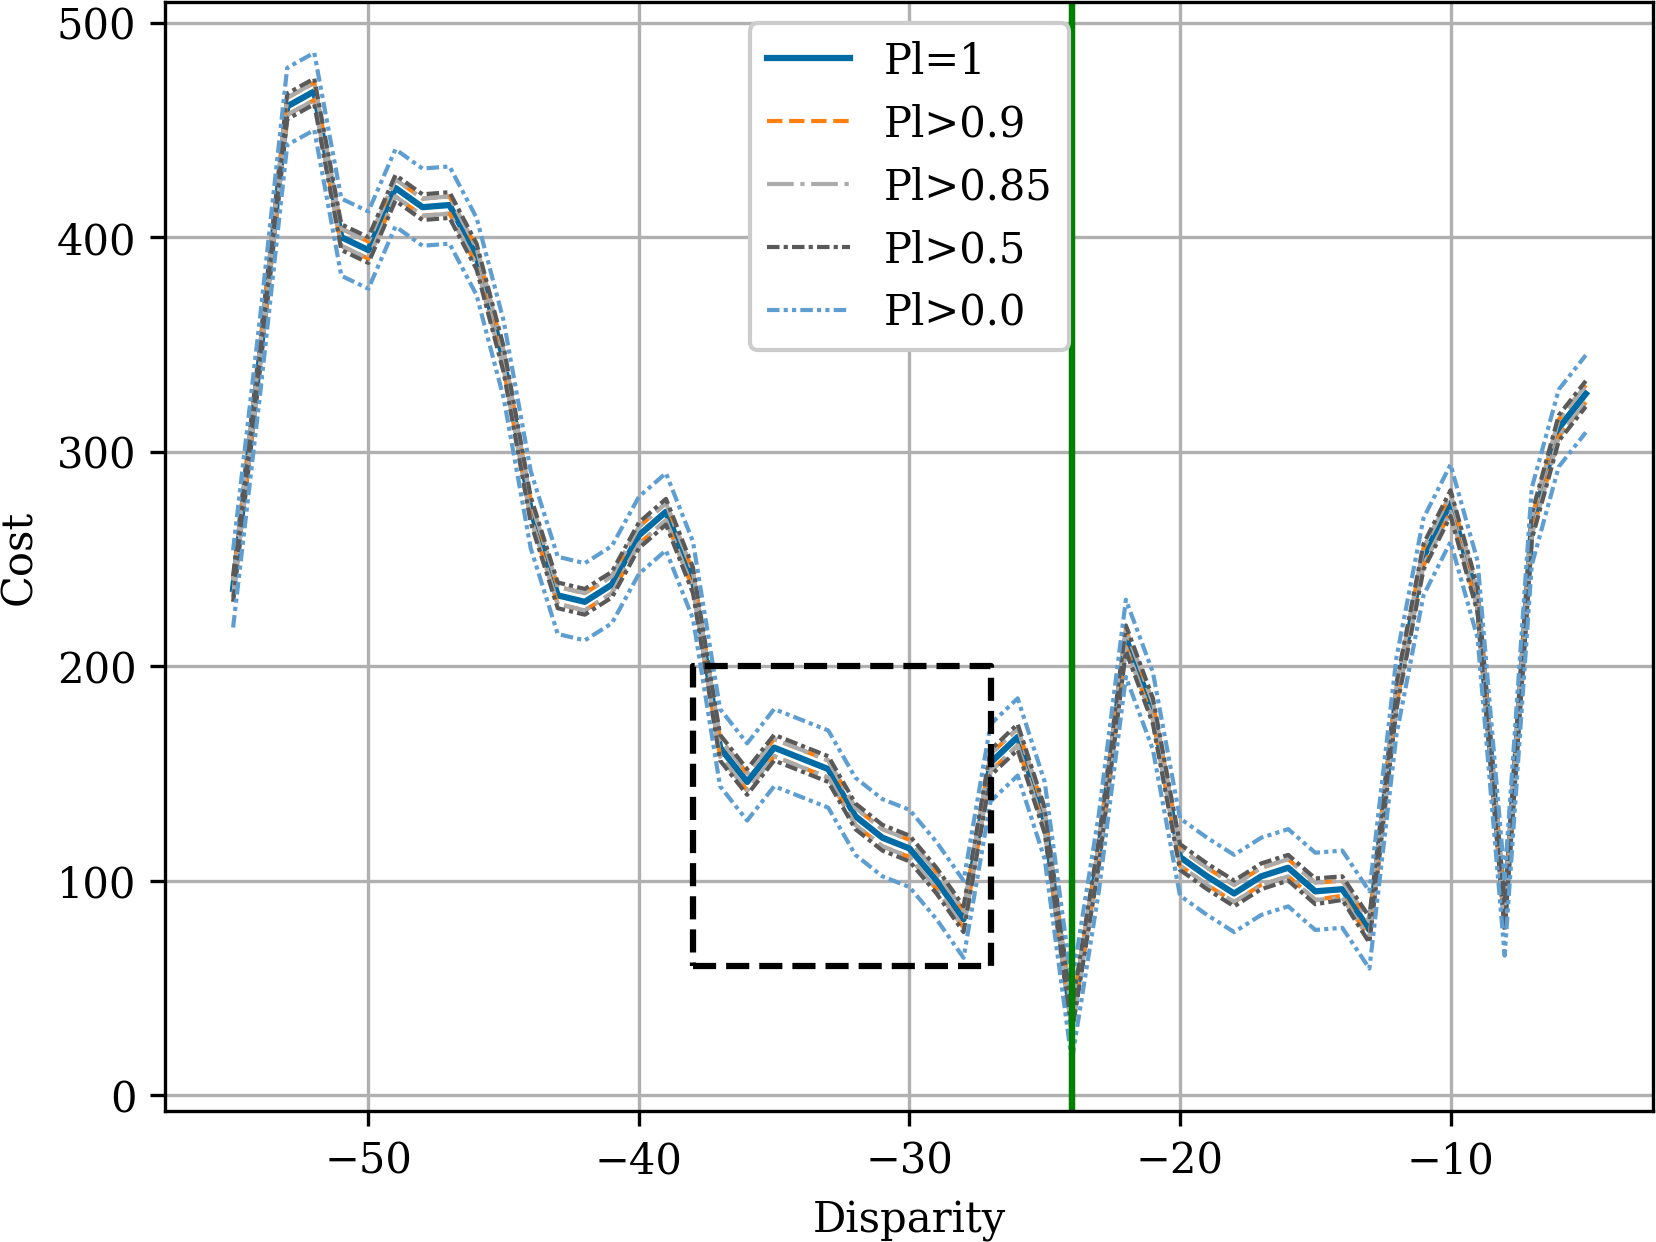
\includegraphics[width=\linewidth]{Images/Chap_4/bel_independence_100_120.png}
        \caption{SAD using the product Copula}
        \label{fig:belief_independence}
    \end{subfigure}\hfill
    \begin{subfigure}{0.48\linewidth}
        \centering
        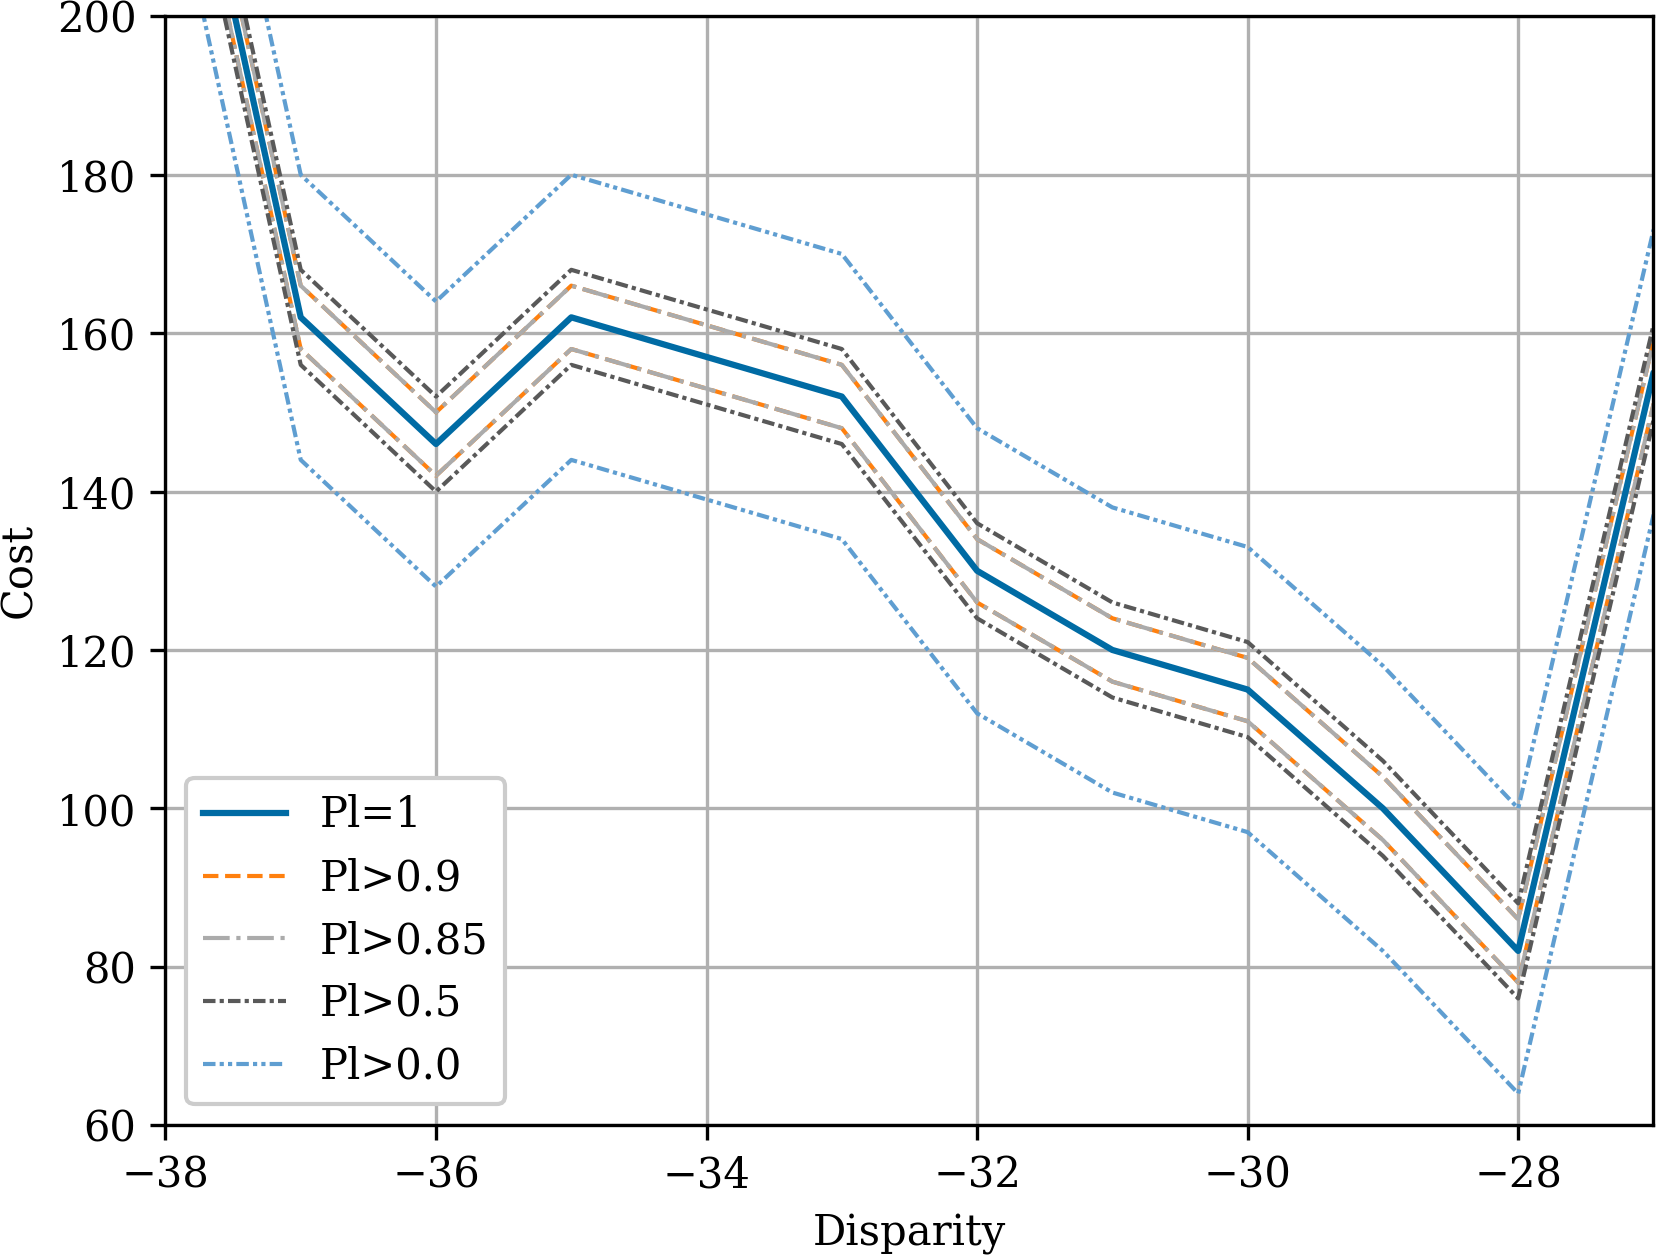
\includegraphics[width=\linewidth]{Images/Chap_4/bel_independence_100_120_zoom.png}
        \caption{Zoom of the rectangle in (a)}
        \label{fig:belief_independence_zoom}
    \end{subfigure}\\
    \begin{subfigure}{0.48\linewidth}
        \centering
        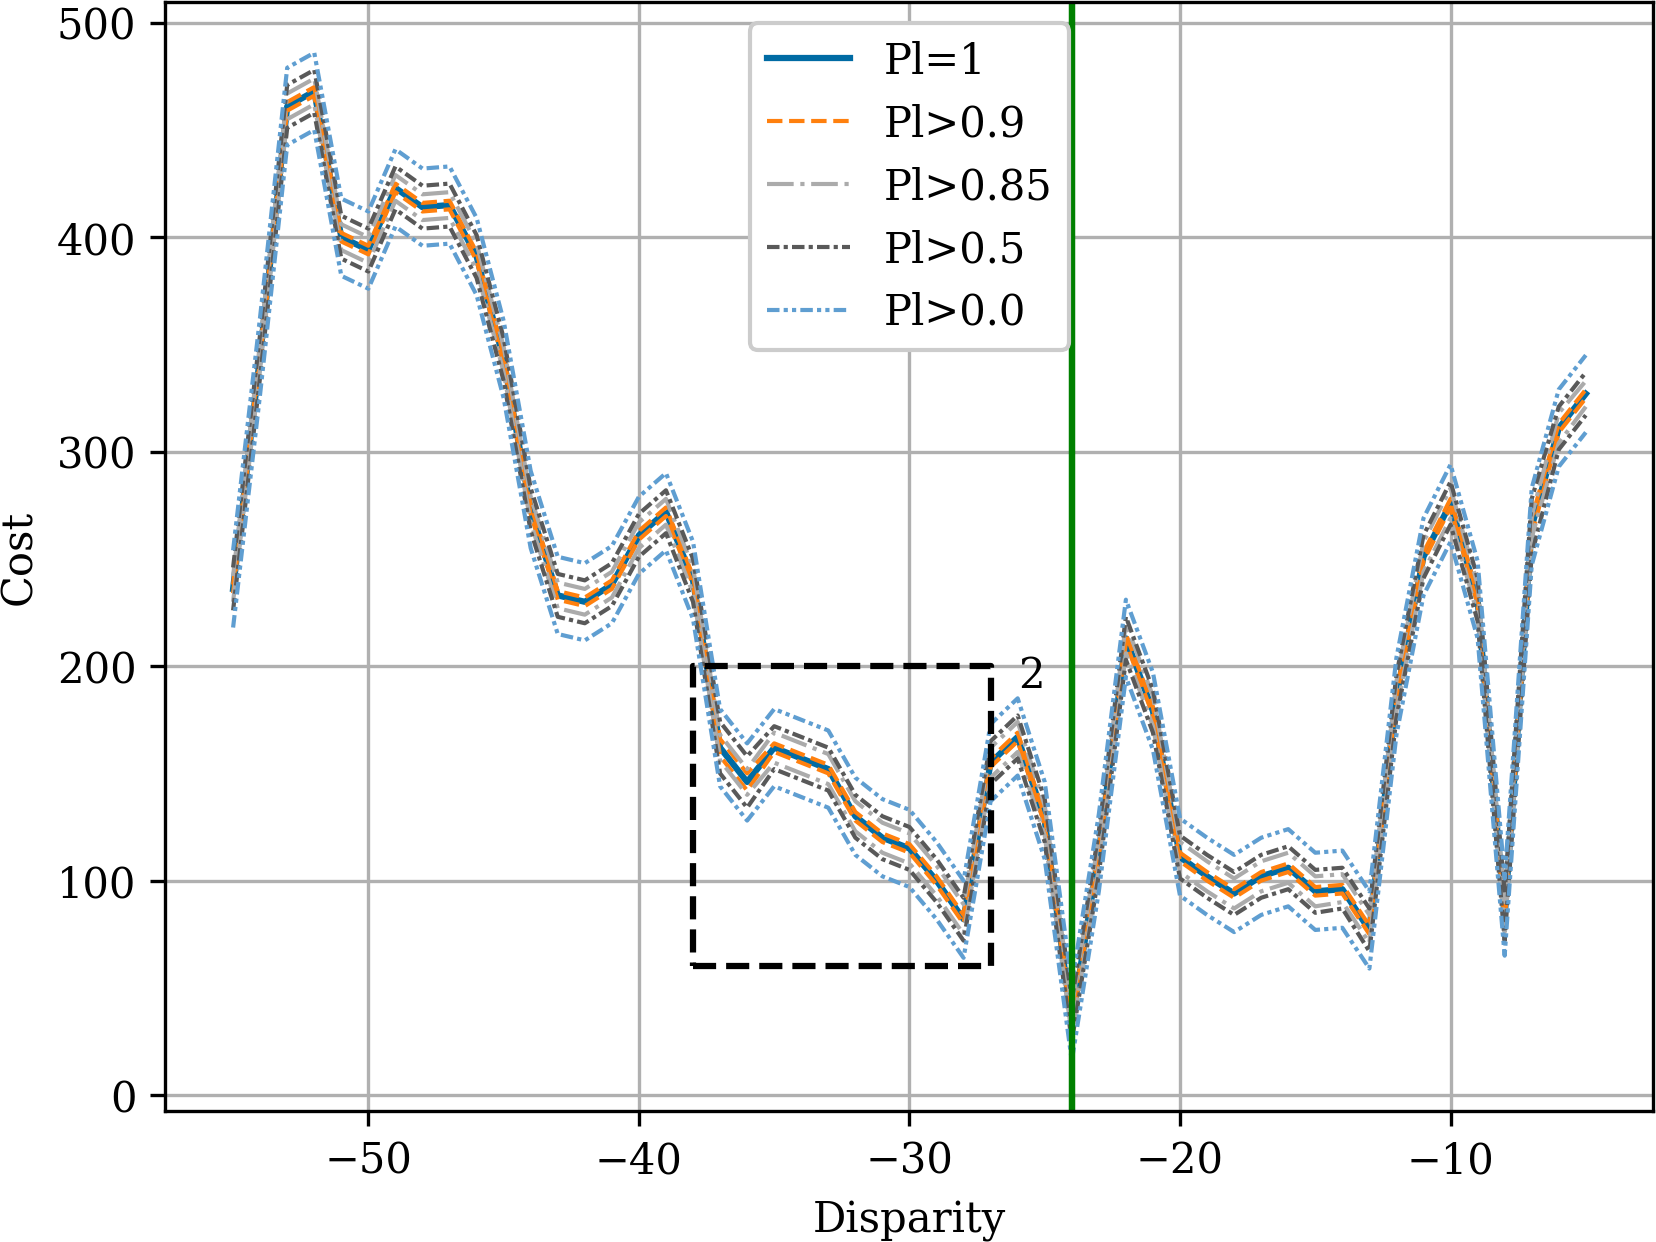
\includegraphics[width=\linewidth]{Images/Chap_4/bel_100_120.png}
        \caption{SAD using the Gaussian Copula}
        \label{fig:belief_gaussian}
    \end{subfigure}\hfill
    \begin{subfigure}{0.48\linewidth}
        \centering
        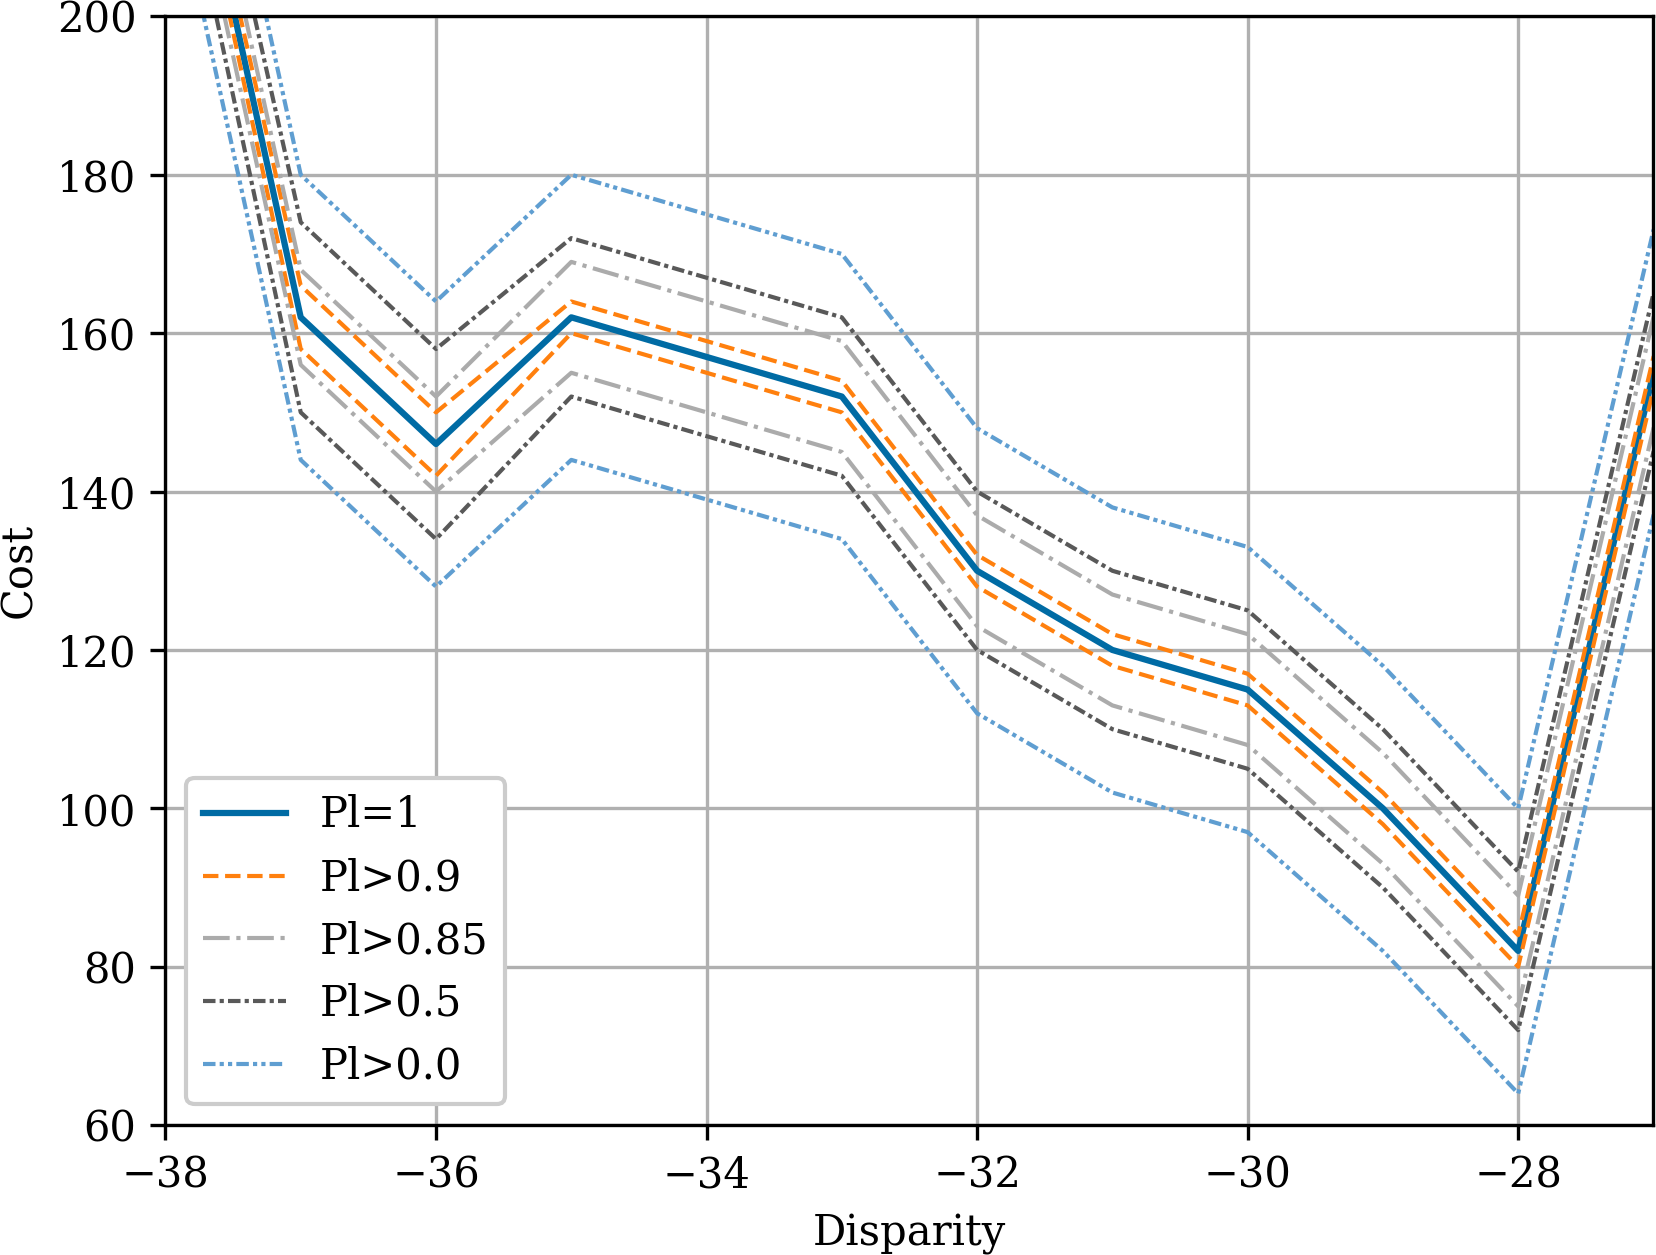
\includegraphics[width=\linewidth]{Images/Chap_4/bel_100_120_zoom.png}
        \caption{Zoom of the rectangle in (c)}
        \label{fig:belief_gaussian_zoom}
    \end{subfigure}
    \caption{Plausibility levels of a cost curve for the product copula $C_\Pi$ and the Gaussian copula $C_R$. The green vertical line represents the true disparity. The figure on the right are a zoom of the black dashed rectangle. From \cite{malinowski_uncertainty_2024}.}
    \label{fig:belief_curves}
\end{figure}

A visualization of different plausibility levels of the SAD cost curve are presented in figure \ref{fig:belief_curves}, computed with the product copula $C_\Pi$ and a Gaussian copula $C_R$. As both copulas assign non-null masses to the same focal sets, their support ($\mathrm{Pl}>0$) is the same. Taking a copula close to the lower Fréchet-Hoeffding bound (which is not a copula for $n>2$), would lead to a different support, as the image of marginal focal set would be assigned a null mass\commanue{ok là tu me perds avec ces deux remarques}. Figures \ref{fig:belief_independence_zoom} and \ref{fig:belief_gaussian_zoom} display the fact that the values covered by the plausibility levels vary with the  copula used. The only exception to this concerns the plausibility level $\gamma=1$, corresponding to the SAD curve without noise\commanue{uncertainty ou sans propagation? Le terme de bruit me gêne un peu}. The plausibility levels $0.85$ and $0.5$ are more concentrated around plausibility level $1$ in the case of the product copula than in the case of the Gaussian copula. Conversely, plausibility level $0.9$ is closer to plausibility level $1$ in the case of the Gaussian copula. This is due to the fact that the Gaussian copula $C_R$ is more co-monotone than the product copula, given the correlation matrix $R$ described in \eqref{eq:correlation}.

\section{Estimating Propagated Credal Sets Using Monte Carlo Sampling}\label{sec:montecarlo}
In order to evaluate the validity of the propagated belief functions, we try to estimate $\M_{robust}$ using Monte Carlo samplings\commanue{ok je suis encore perdue, ce qu'on a calculé avant ne suffit pas ?? donc conclusion puis on explique ce qui manque et bam nouvelle section. Et cerise sur le gateau, le lien est le fameux chapitre 3}. We first generate probability distributions belonging in the marginal credal sets. This sampling is not random as we generate probability distributions in such a way that the probability range on events imposed by the marginal possibility distributions is uniformly covered. We also make sure that lower and upper bounds on events are all reached at least once, in order to include ``extreme'' distributions in our simulations. Once every marginal probability distribution of every pixel used to compute a cost curve has been sampled, we can generate random samples from their joint distribution. We thus generate samples from the copula and marginals as detailed in section \ref{sec:sampling_copula}. This yields noised version of patches from the left images, where the noised samples dependency is modeled by the provided copula. Finally, we compute the cost curves using those random images, giving us Monte Carlo samples of the SAD cost curves for a given copula\commanue{combien de samples?}.

Note that we could simulate a single version of the noised pair of images, but that would require to sample from a copula of very large dimension (the number of pixels in both images). This is not realistically feasible, even thought it would ensure that the same version of noised pixels are used in all cost curves (or in other words, for a single draw, the noised intensities will not change depending on the cost curve computed). We instead generate noise samples for each row separately: noised values of pixels will not change during the evaluation of a cost curve for different disparities, or between the cost curves of pixels of the same row. However, their values might change between cost curves of pixels belonging to different rows. For instance, let's consider a pixel $p=(row,~col)\in I_L$ for which we computed a noised intensity $i_p$. Then we will use the same noised value $i_p$ of intensity when computing the SAD of every pixel $q=(row,~col')\in I_L$. But when computing the SAD of every pixel $q=(row-1,~col')\in I_L$, we will use a different Monte Carlo draw for the value $i_p$, which will stay the same for every pixel of row $row-1$. Because we draw a high number of Monte Carlo draws ($10,000$) for each row, the effect of this of proceeding should not be noticeable. 

Monte Carlo draws using the Gaussian copula and marginals credal sets of \ref{eq:pixel_possibility} are plotted in figures \ref{fig:montecarlo_gauss_100_120} and \ref{fig:montecarlo_gauss_200_150}. Different plausibility levels, similar to those of figures \ref{fig:belief_curves}, also appear for comparison. The support envelopes from plausibility levels $\mathrm{Pl}>0$ correctly contain all Monte Carlo samplings for all considered copulas. We can observe in Figure \ref{fig:montecarlo_gauss_200_150_zoom2} that plausibility levels sometimes fail to correctly grasp the fluctuations of the dispersion of the samples, even though they seem to correctly contain Monte Carlo samples. For instance, Monte Carlo draws are first dense around disparity $-37$, then seem to spread around $-35$, and finally regather around disparity $-32$. The plausibility envelopes are more regular in this disparity range. This illustrates the fact the ``true'' point-wise credal $\M_{robust}$ set described in section \ref{sec:robust_method} and approximated with Monte Carlo samples is different from that the joint credal set $\M_{mass}$ from section \ref{sec:joint_mass}. Although some differences persist between those sets, Figure \ref{fig:montecarlo_gauss_100_120_zoom2} or \ref{fig:montecarlo_gauss_200_150_zoom2} suggest that Monte Carlo simulations can correctly estimate the point-wise credal set $\M_{robust}$ by joining belief functions using a copula as in equation \eqref{eq:joint_mass}. This is furthermore justified by the  quantitative analysis presented in Table \ref{tab:Coverage}, where the proportion of Monte Carlo samplings contained inside the plausibility envelopes, is computed for different plausibility levels $\gamma$. We will call this proportion ``coverage''. The coverage for figures \ref{fig:montecarlo_gauss_100_120} and \ref{fig:montecarlo_gauss_200_150} are presented in the first and second rows of Table \ref{tab:Coverage} respectively. The global coverage over the whole left image is presented in the last row of the table. The coverage is always $100\%$ for $\gamma=0$, which indicates that every sample is contained inside the support envelopes. \todoroman{Je pense que ce que je dis ensuite est faux. Le coverage ne donne pas d'indication sur les plausibility estimées, car celles ci ne retranscrivent pas une fréquence mais seulement un niveau de croyance. Comment donner une interprétation correcte de la densité?} As envelopes are defined as lower and upper bounds of the focal sets with a plausibility superior to $\gamma$, the coverage should be superior to $1-\gamma$, which is indeed the case \commanue{conclusion ?}.

\begin{figure}
    \centering
    \begin{subfigure}{1\linewidth}
        \centering
        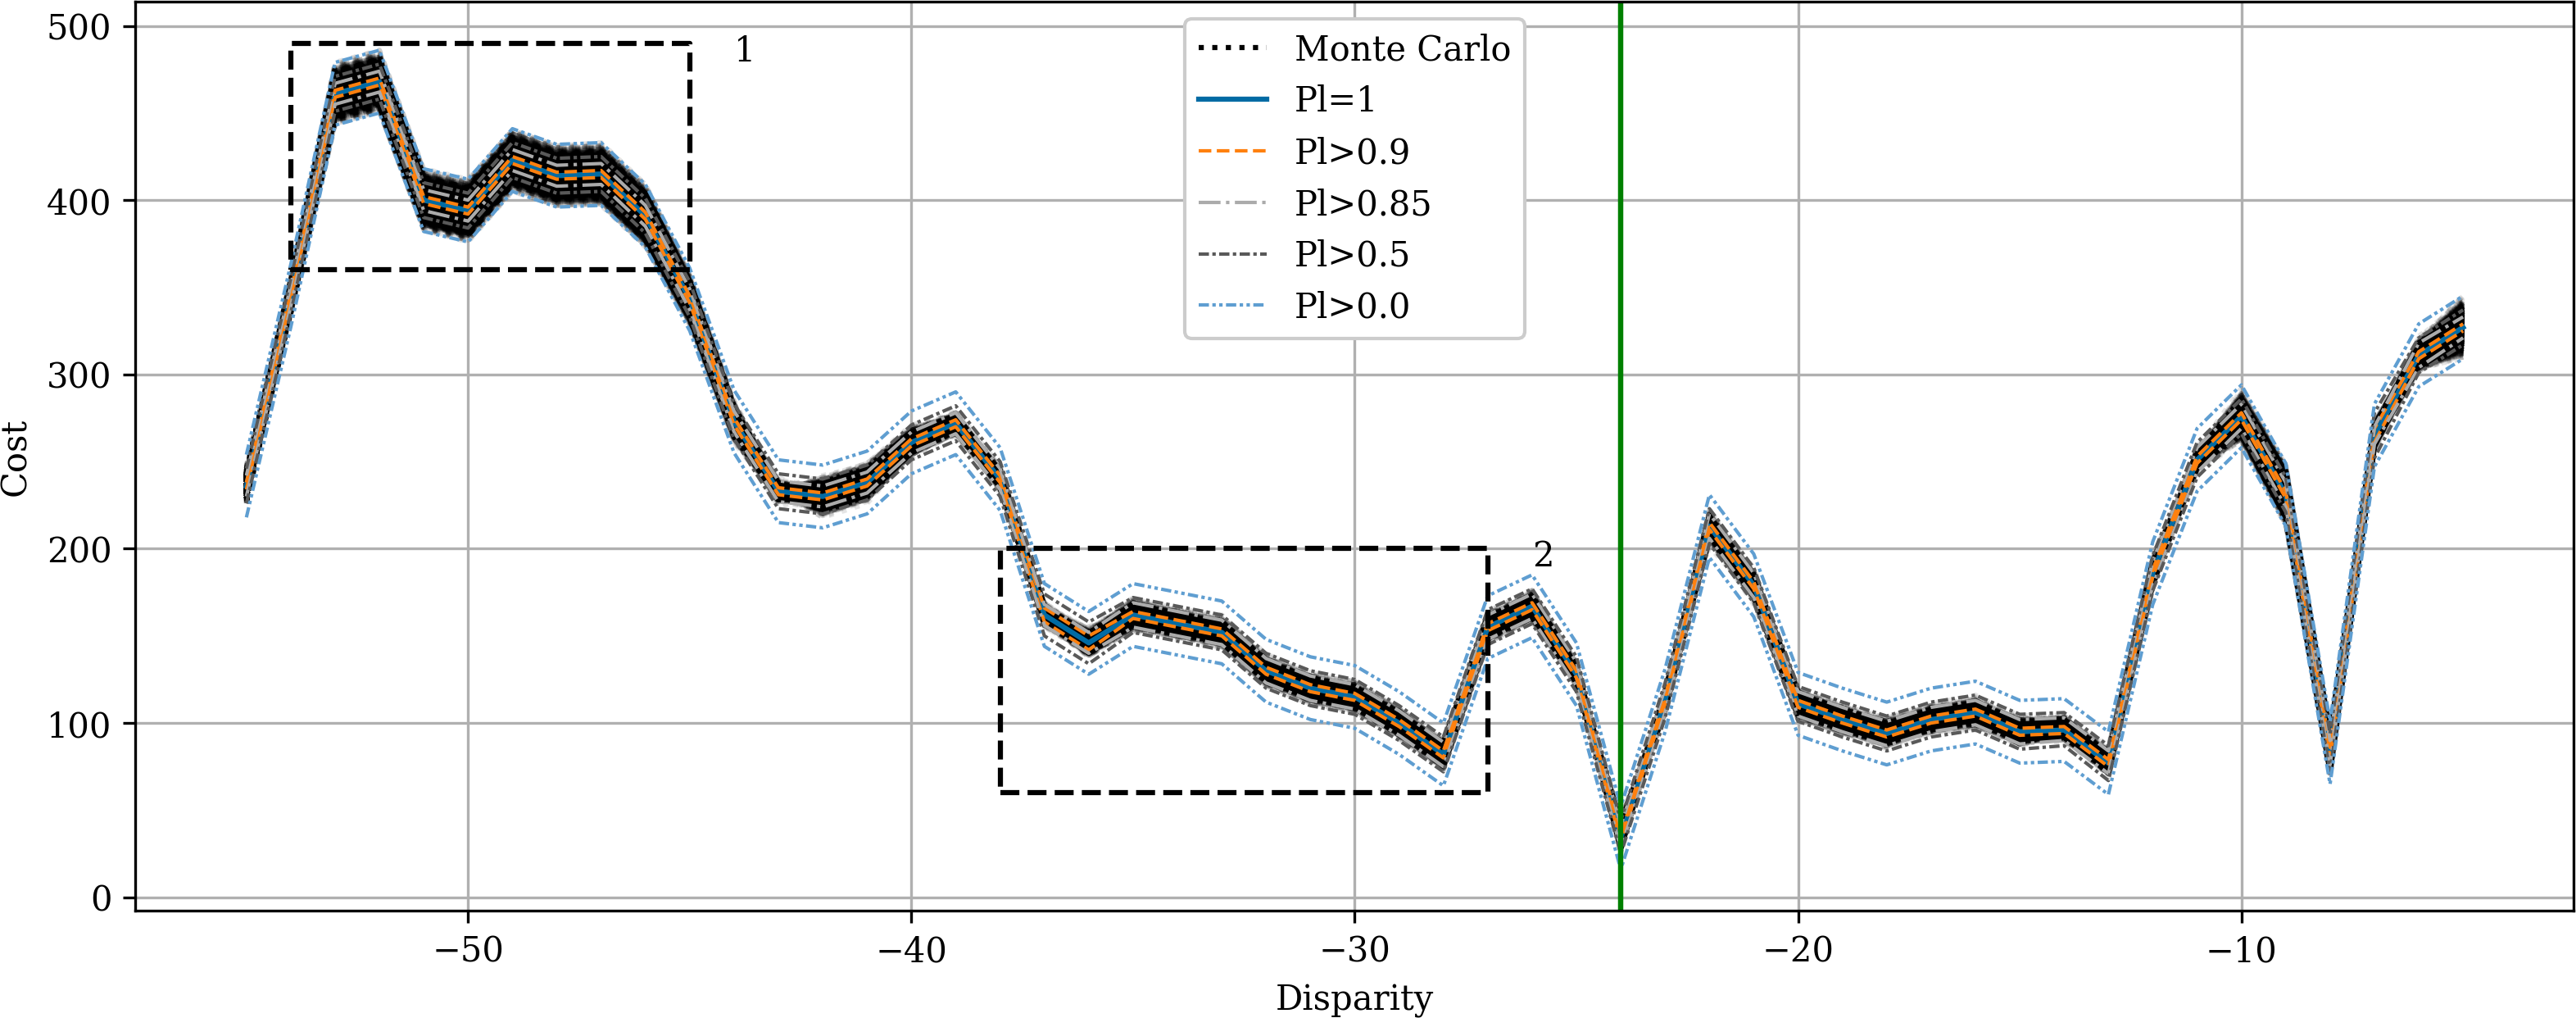
\includegraphics[width=\linewidth]{Images/Chap_4/cost_curve_100_120.png}
        \caption{Plausibility levels and Monte Carlo sampling using a Gaussian copula}
        \label{fig:montecarlo_gauss_100_120_large}
    \end{subfigure}\\
    \begin{subfigure}{0.45\linewidth}
        \centering
        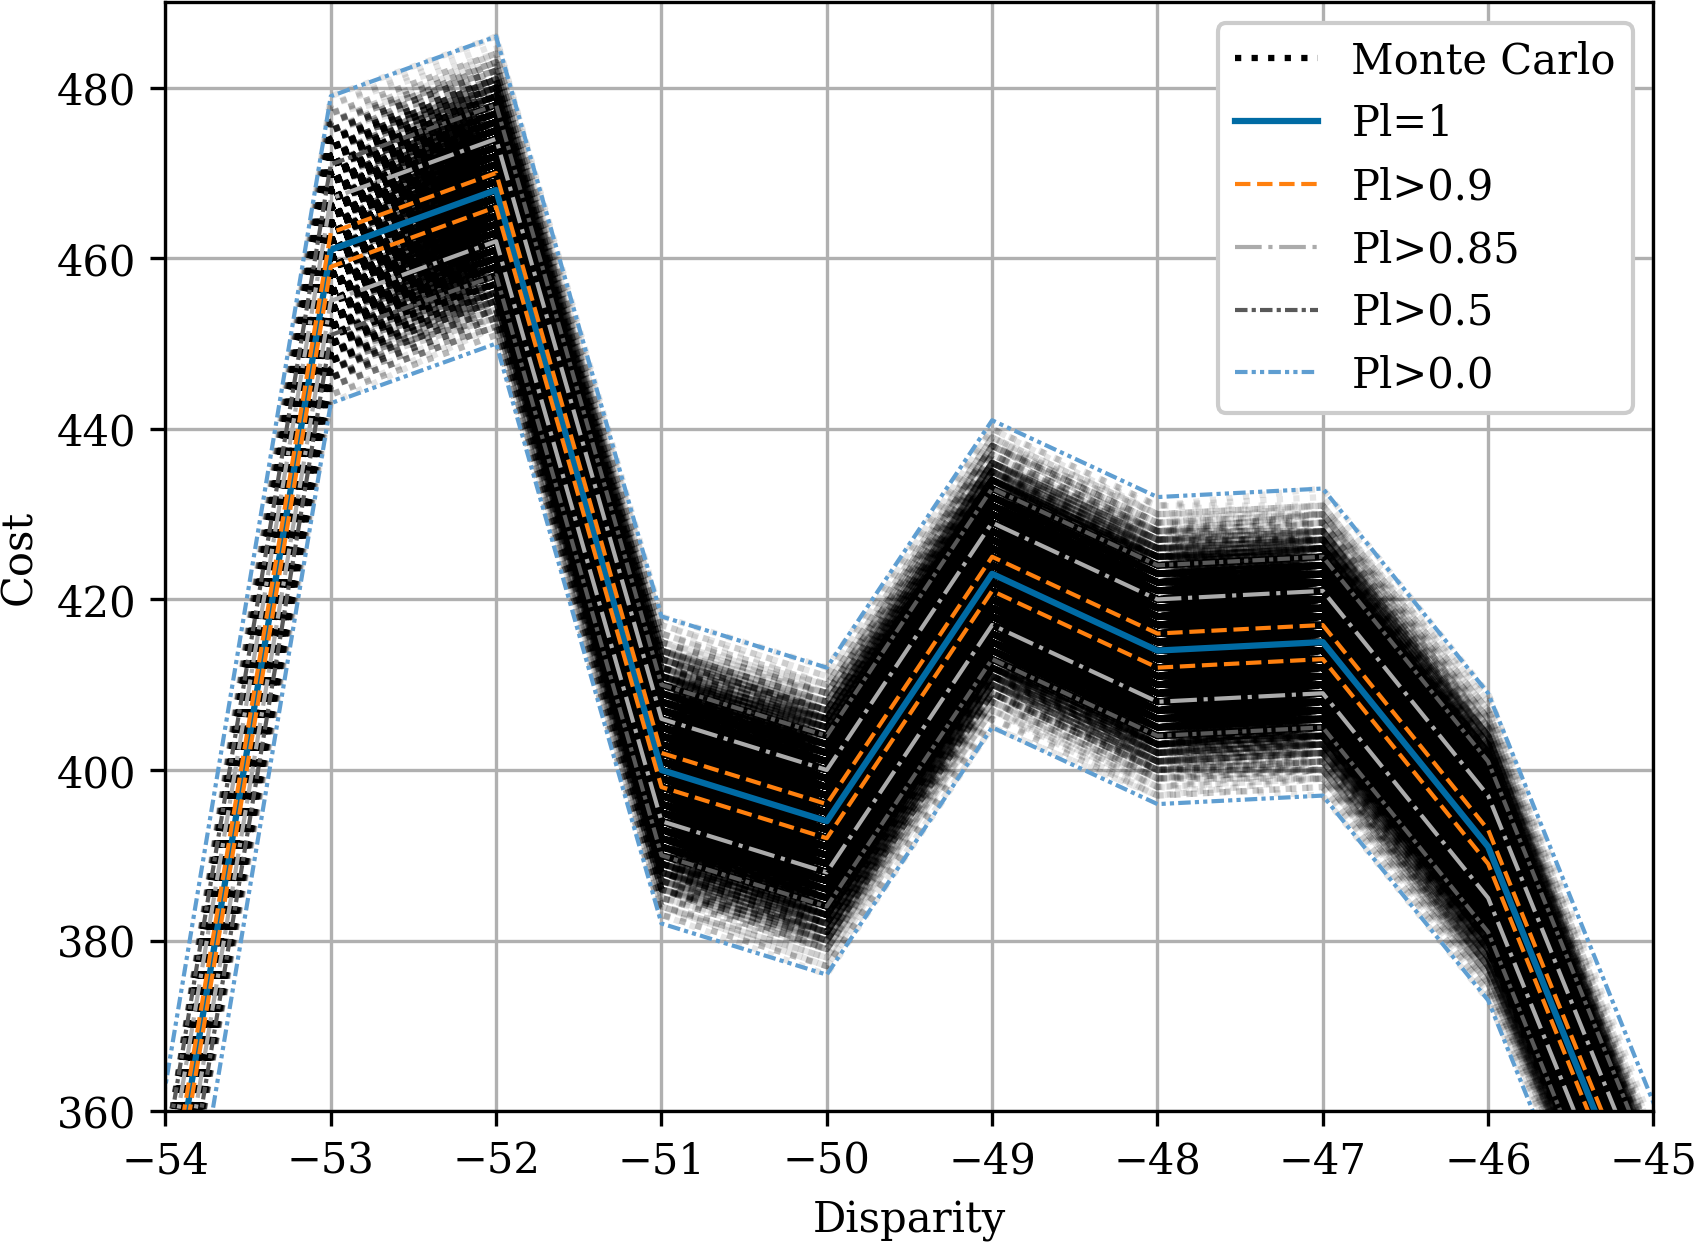
\includegraphics[width=\linewidth]{Images/Chap_4/cost_curve_100_120_zoom1.png}
        \caption{Zoom over the first rectangle}
        \label{fig:montecarlo_gauss_100_120_zoom1}
    \end{subfigure}\hfill
    \begin{subfigure}{0.45\linewidth}
        \centering
        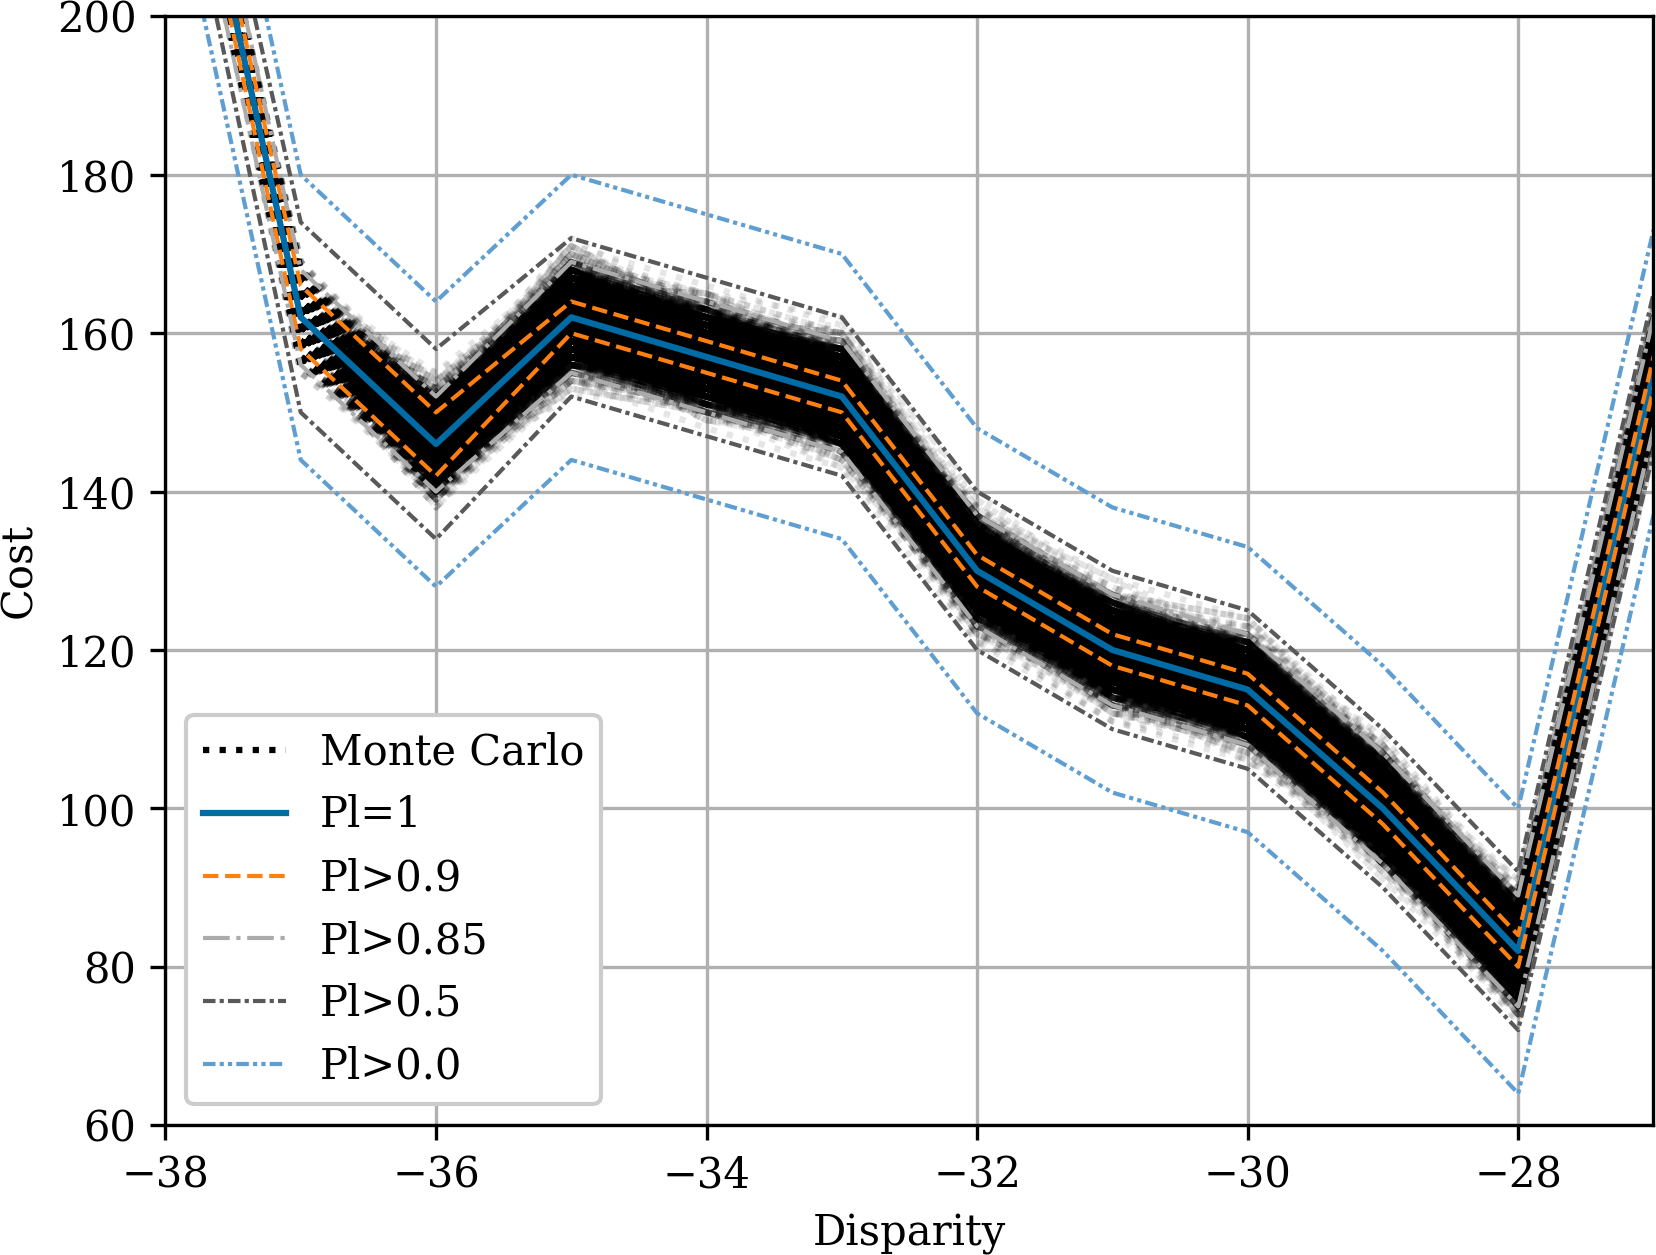
\includegraphics[width=\linewidth]{Images/Chap_4/cost_curve_100_120_zoom2.png}
        \caption{Zoom over the second rectangle}
        \label{fig:montecarlo_gauss_100_120_zoom2}
    \end{subfigure}
    \caption{Plausibility levels and Monte Carlo sampling for a pixel of the left image. From \cite{malinowski_uncertainty_2024}.}
    \label{fig:montecarlo_gauss_100_120}
\end{figure}

\begin{figure}
    \centering
    \begin{subfigure}{\linewidth}
        \centering
        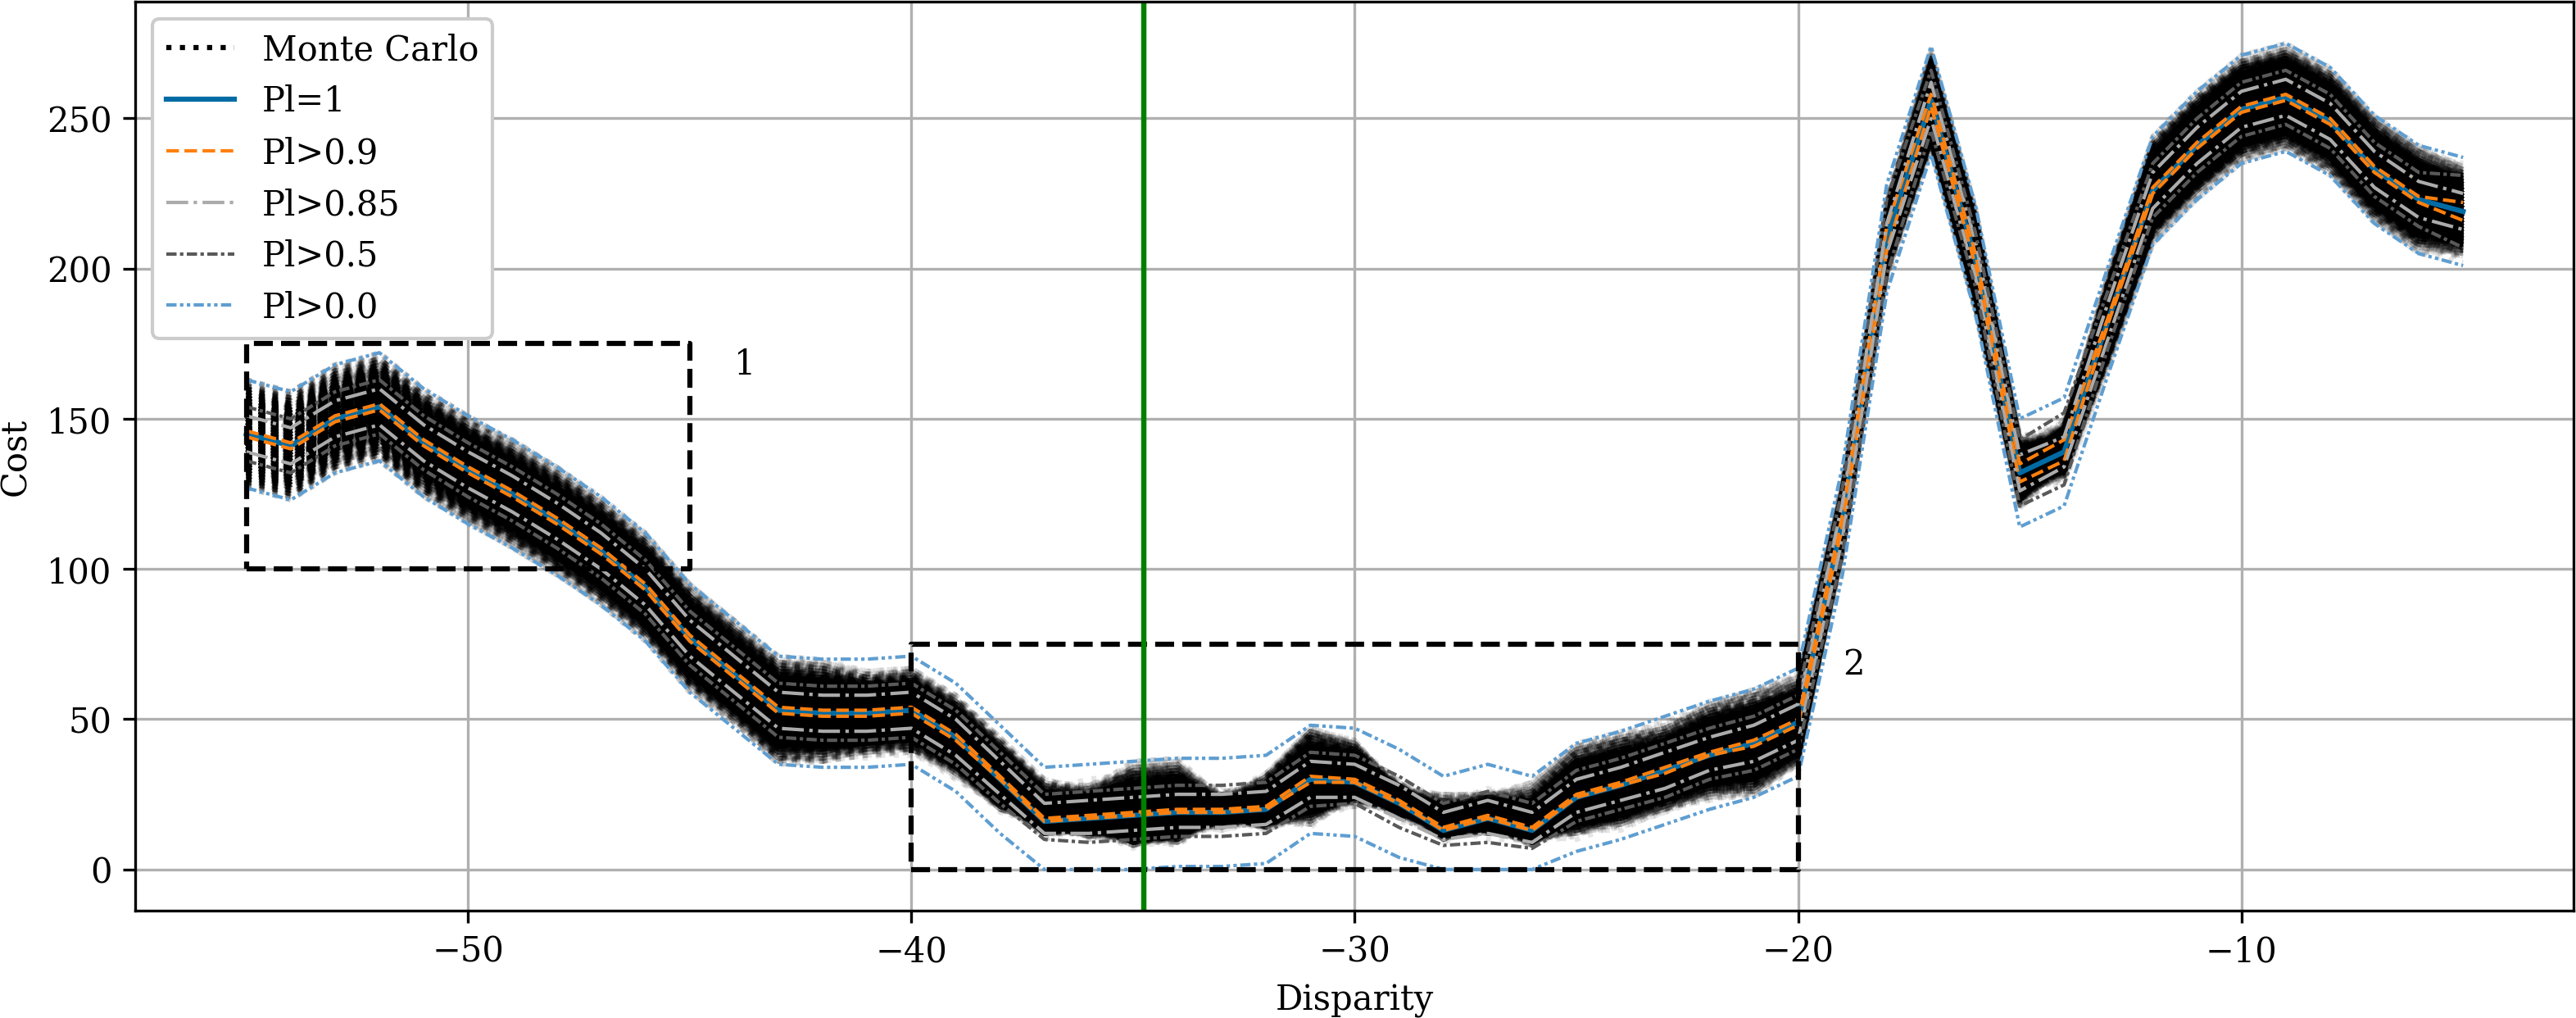
\includegraphics[width=\linewidth]{Images/Chap_4/cost_curve_200_150.png}
        \caption{Plausibility levels and Monte Carlo sampling using a Gaussian copula}
        \label{fig:montecarlo_gauss_200_150_large}
    \end{subfigure}\\
    \begin{subfigure}{0.45\linewidth}
        \centering
        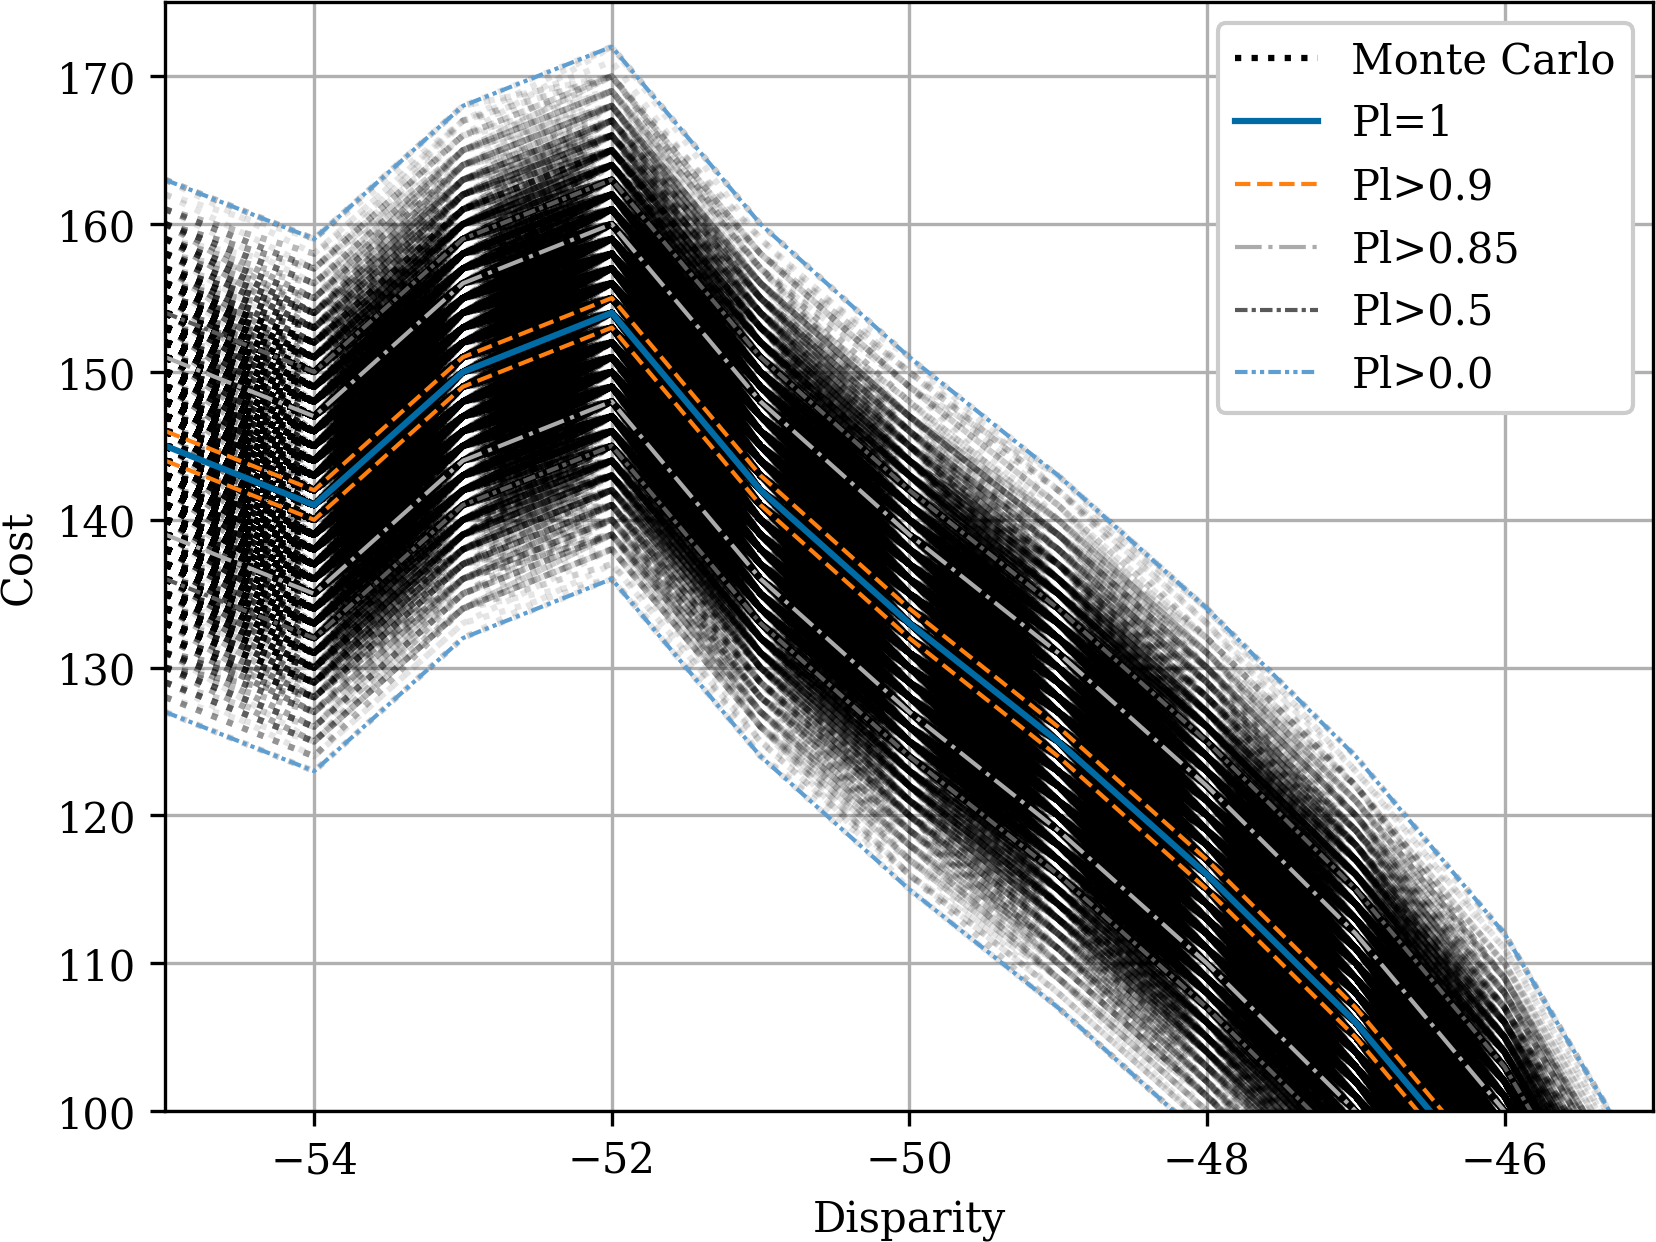
\includegraphics[width=\linewidth]{Images/Chap_4/cost_curve_200_150_zoom1.png}
        \caption{Zoom over the first rectangle}
        \label{fig:montecarlo_gauss_200_150_zoom1}
    \end{subfigure}
    \hfill
    \begin{subfigure}{0.45\linewidth}
        \centering
        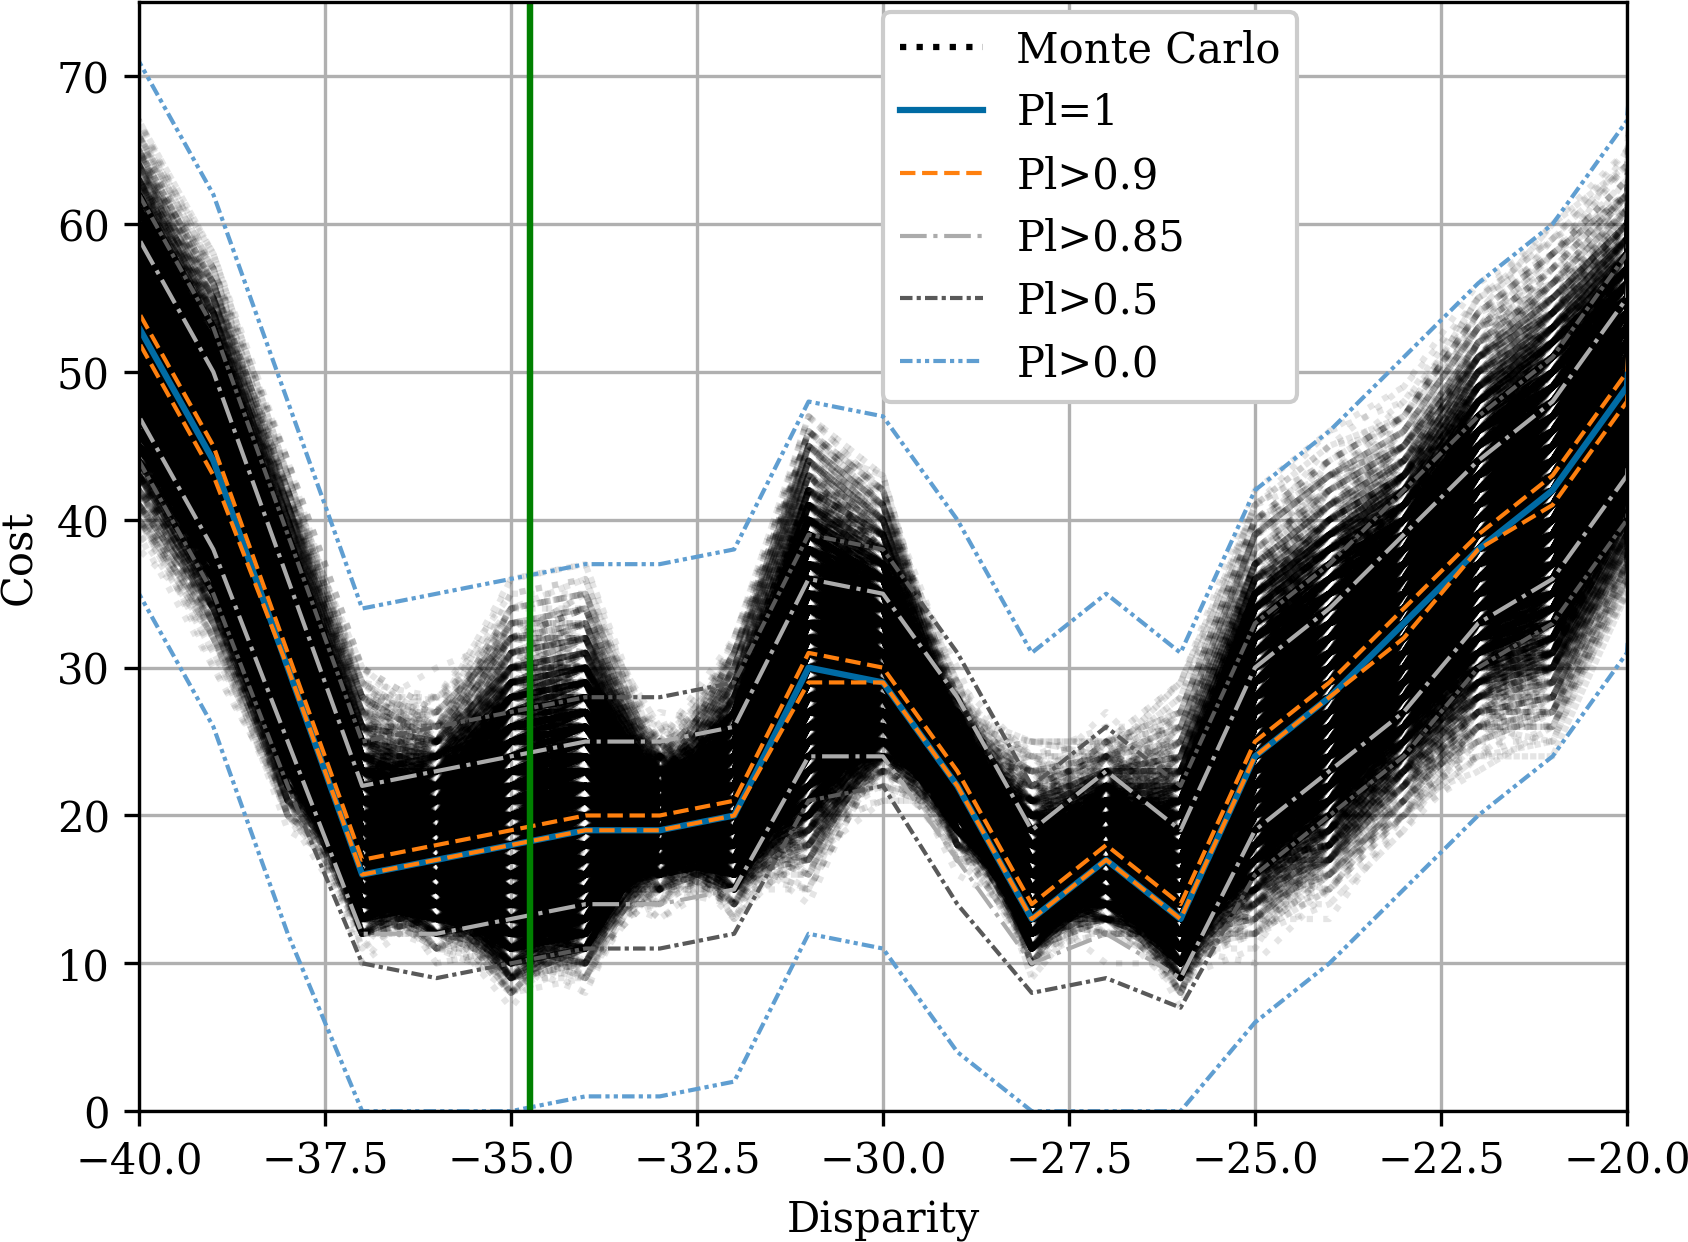
\includegraphics[width=\linewidth]{Images/Chap_4/cost_curve_200_150_zoom2.png}
        \caption{Zoom over the second rectangle}
        \label{fig:montecarlo_gauss_200_150_zoom2}
    \end{subfigure}
    \caption{Plausibility levels and Monte Carlo sampling for a pixel of the left image.  From \cite{malinowski_uncertainty_2024}.}
    \label{fig:montecarlo_gauss_200_150}
\end{figure}

\begin{table}[ht]
\centering
\begin{tabular}{|c|c|c|c|c|}
\hline
\rowcolor[HTML]{C0C0C0}
$p=(row,col)$ & $\gamma=0.9$  & $\gamma=0.85$ & $\gamma=0.5$  & $\gamma=0$   \\ \hline
\cellcolor[HTML]{C0C0C0}$(100,~120)$     & $64,5\%$ & $94,5\%$ & $99,0\%$ & $100\%$ \\ \hline
\cellcolor[HTML]{C0C0C0}$(200,~150)$     & $30,0\%$ & $82,6\%$ & $95,2\%$ & $100\%$ \\ \hline
\cellcolor[HTML]{C0C0C0}Global        & $41,1\%$ & $87,6\%$ & $96,8\%$ & $100\%$ \\ \hline
\end{tabular}
\caption{Average coverage for various plausibility levels $\gamma$ and for different pixels $p$ of the left image.}\label{tab:Coverage}
\end{table}

\begin{figure}[ht]
    \centering
    \begin{subfigure}{0.48\linewidth}
        \centering
        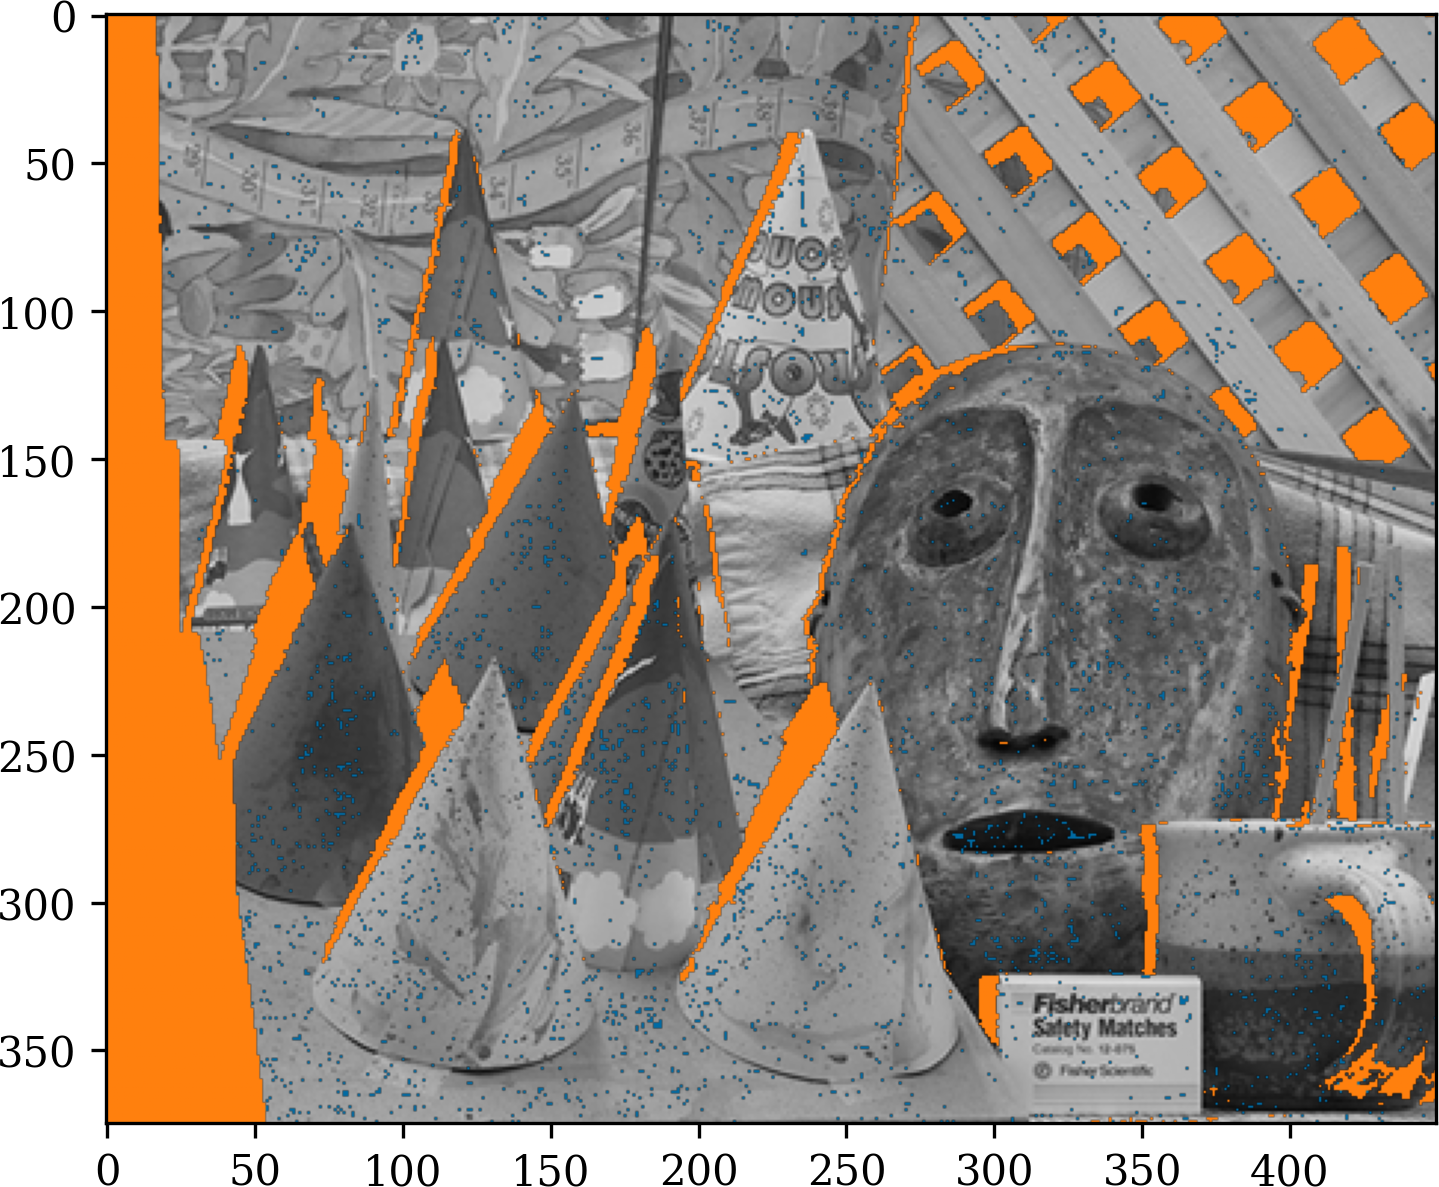
\includegraphics[width=\linewidth]{Images/Chap_4/Improvements_Pl=0.9.png}
        \caption{$\gamma=0.9,~\Delta s_\gamma=4.05\%$}
        \label{fig:improvements_a}
    \end{subfigure}
    \begin{subfigure}{0.48\linewidth}
        \centering
        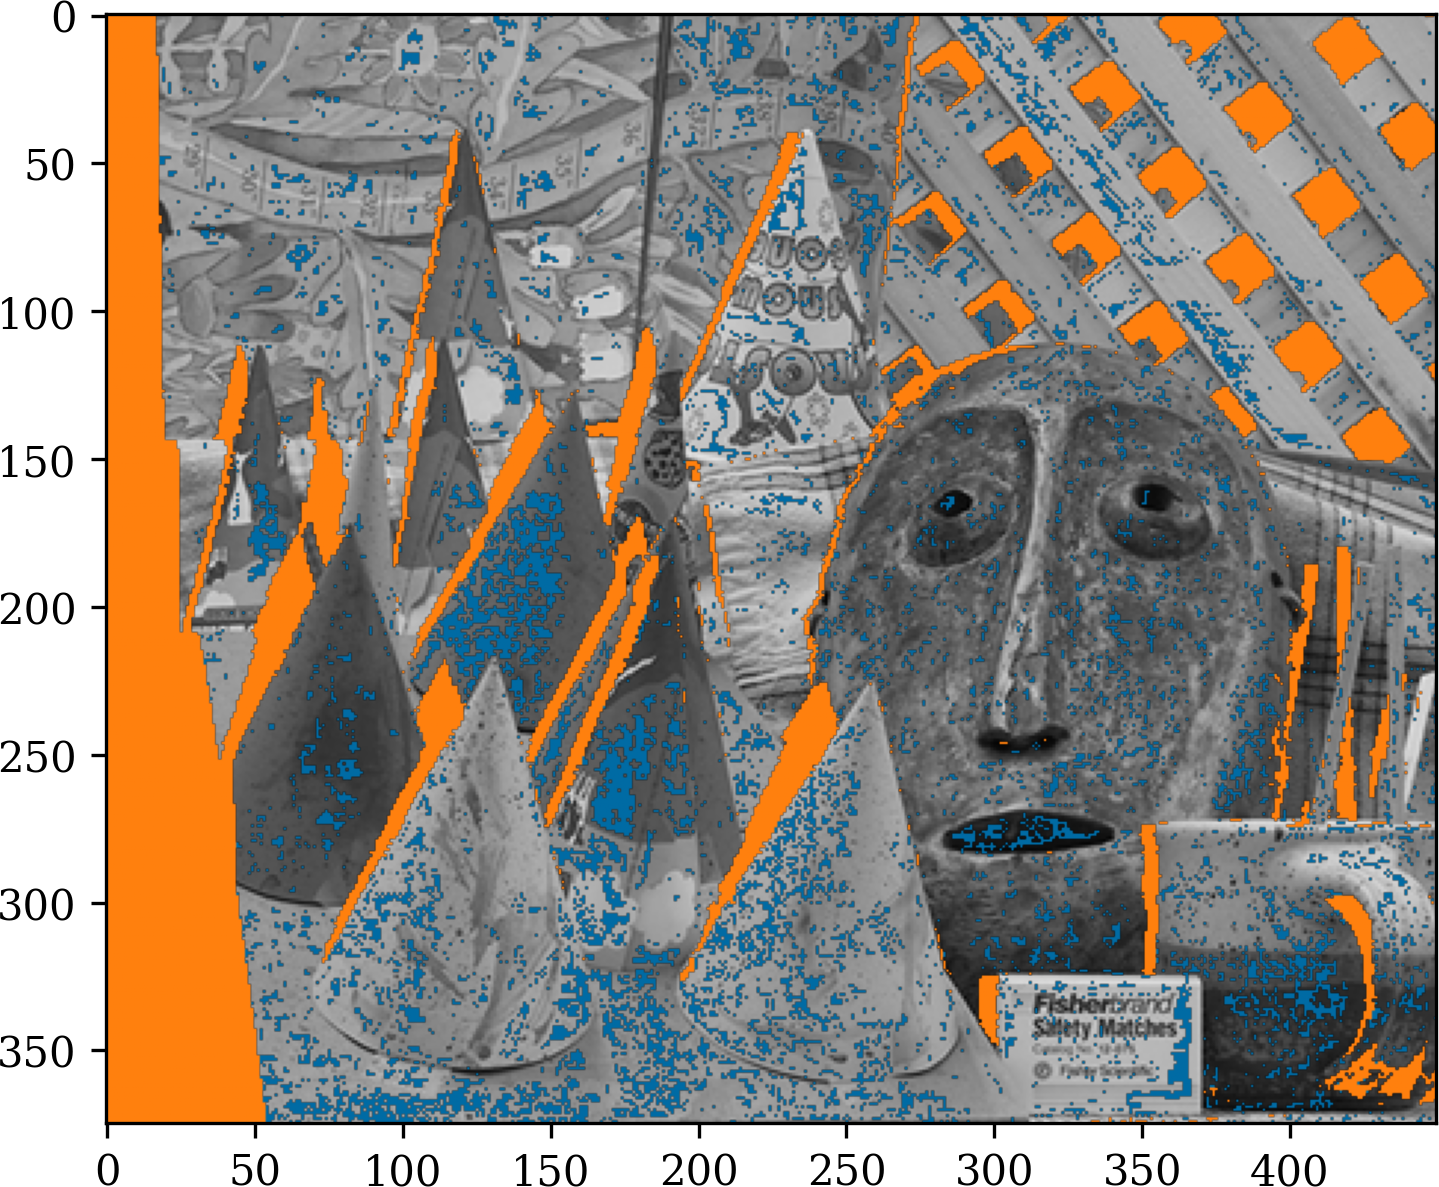
\includegraphics[width=\linewidth]{Images/Chap_4/Improvements_Pl=0.85.png}
        \caption{$\gamma=0.85,~\Delta s_\gamma=16.11\%$}
        \label{fig:improvements_b}
    \end{subfigure}\\
    \begin{subfigure}{0.48\linewidth}
        \centering
        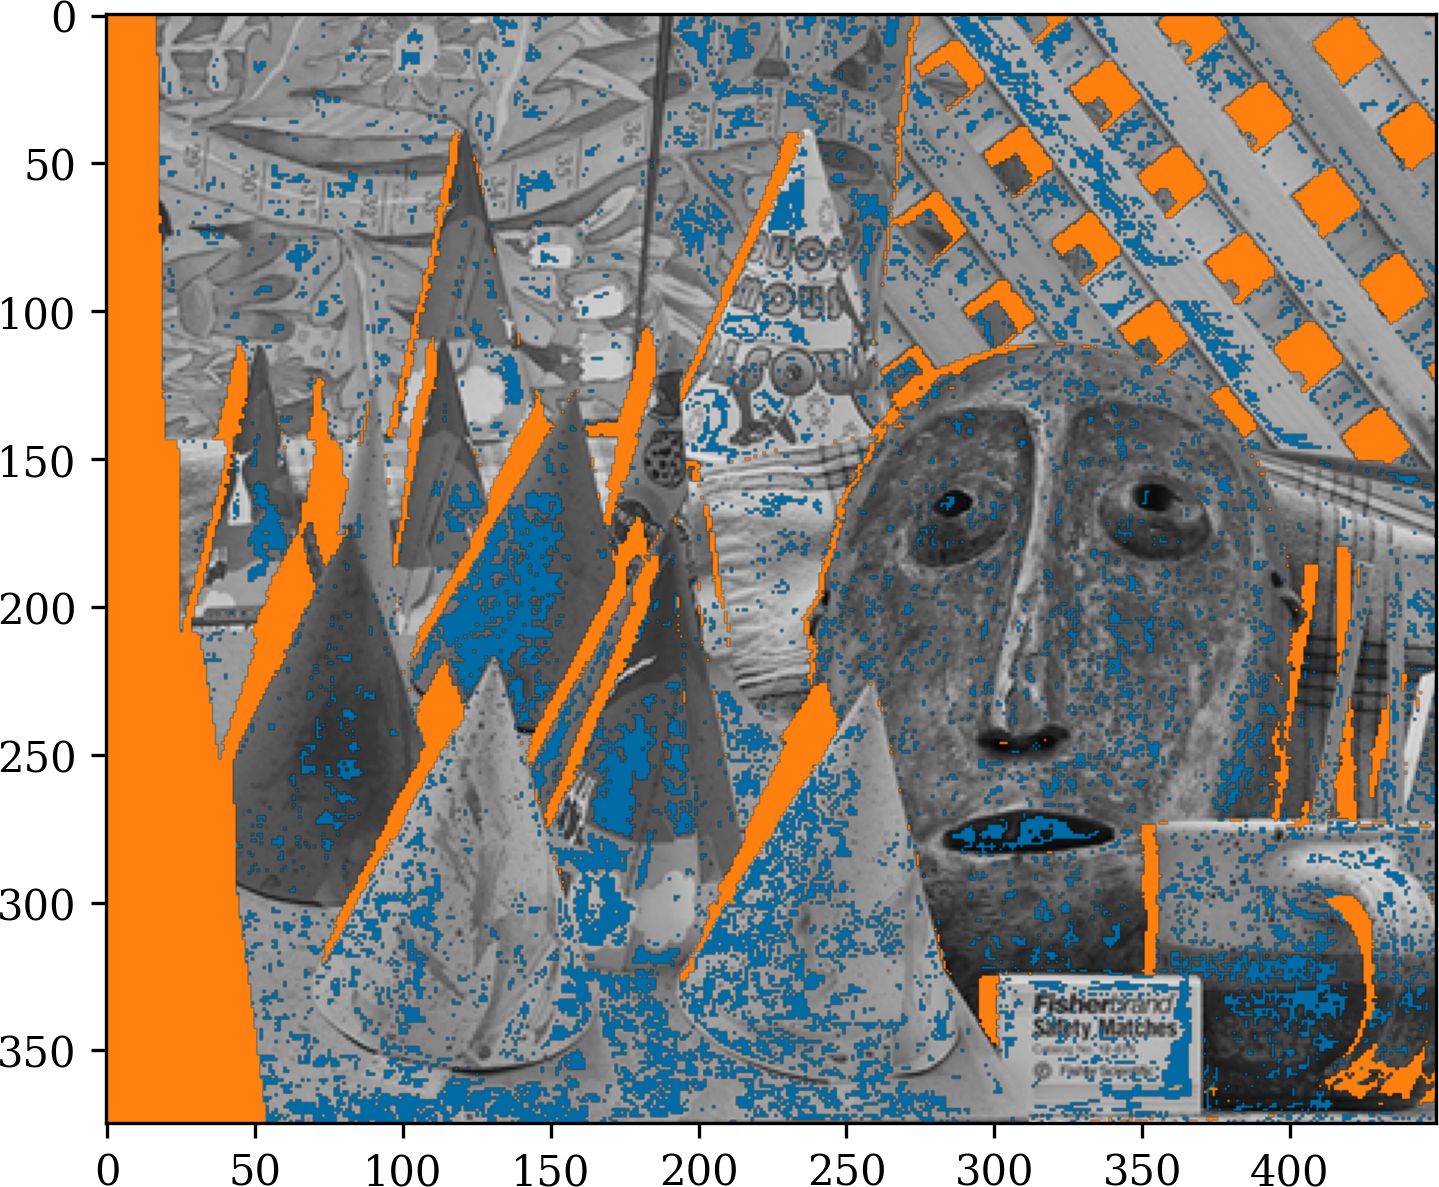
\includegraphics[width=\linewidth]{Images/Chap_4/Improvements_Pl=0.5.png}
        \caption{$\gamma=0.5,~\Delta s_\gamma=21.41\%$}
        \label{fig:improvements_c}
    \end{subfigure}
    \begin{subfigure}{0.48\linewidth}
        \centering
        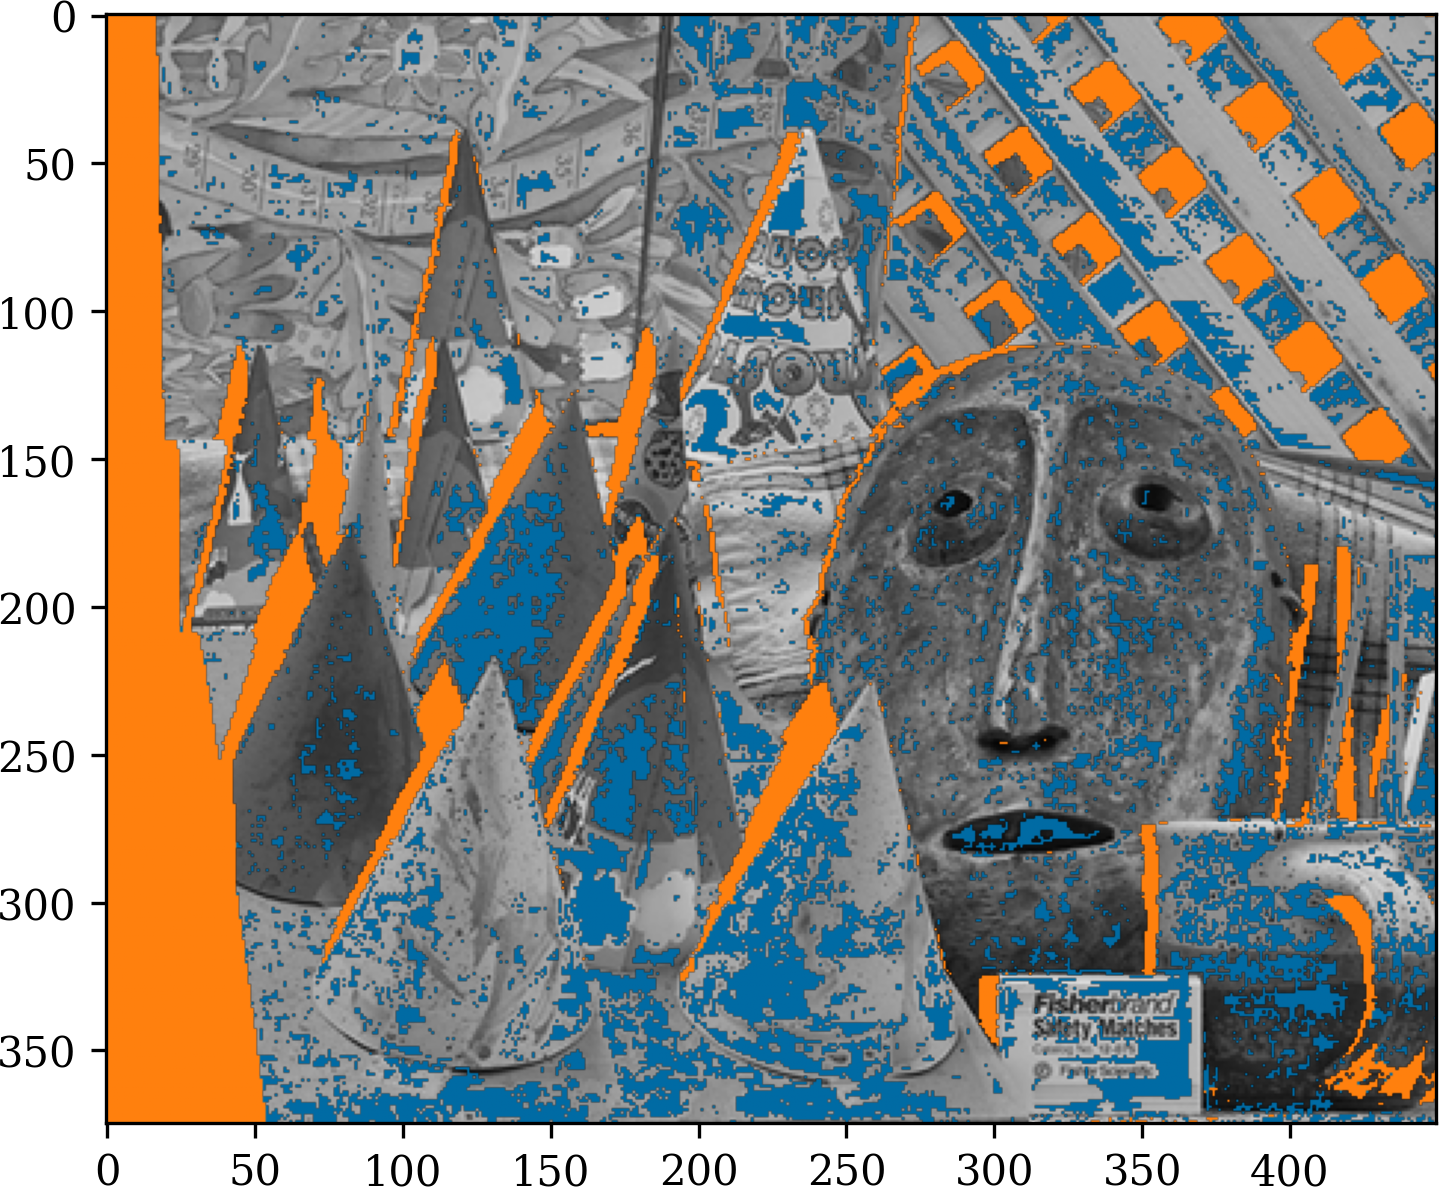
\includegraphics[width=\linewidth]{Images/Chap_4/Improvements_Pl=0.0.png}
        \caption{$\gamma=0,~\Delta s_\gamma=28.87\%$}
        \label{fig:improvements_d}
    \end{subfigure}
    \caption{Spatial disposition of potential improvements for different values of $\gamma$. Pixels with potential improvements appear in blue. Occluded pixels, for which a correct disparity does not exist, appear in orange. Grayscale left image is displayed on the background. From \cite{malinowski_uncertainty_2024}.}
    \label{fig:improvements}
\end{figure}

\section{Leveraging Confidence Envelopes for Potential Improvements}

Knowing the uncertainty, in our case represented as confidence envelopes, can provide valuable insights into potential matches. This section outlines observations suggesting that incorporating this information can enhance the performance of stereo-matching algorithms\commanue{donc on va bien jusqu'à la disparité, c'était pas dans l'intro}.

A common metric for evaluating stereo algorithm performance is the proportion of pixels $(row, col)$ for which the absolute difference between the true disparity and the predicted disparity is less than one pixel. This metric is used as we only consider integer disparities, but the ground truth disparity can be any real number in the disparity range. We thus consider a disparity to be ``correct'' if it is less than one pixel away from the true disparity. With this definition, there can be two ``correct'' disparities for every cost curve, which is inherent to the limited number of disparities one can consider\commanue{il est 23h passé mais là je comprends pas}. Let $d_{\mathrm{true}}(row, col)$ denote the true disparity and $\tilde{d}(row, col) = \arg \min_d \SAD(row, col, d)$ be the estimated disparity at pixel $(row, col)$. The score \( s \) is defined as:
\begin{equation}
    s = \frac{\#\{(row, col) \text{ such that } |d_{\mathrm{true}}(row, col) - \tilde{d}(row, col)| < 1\}}{\#\{(row, col)\}}\,.
\end{equation}

For a given confidence level $\gamma \in [0, 1]$ and a pixel $(row, col)$, we define the set of potential disparities $D_\gamma^{row, col}$ as:
\begin{equation}
    D_\gamma^{row, col} = \{d \mid \underline{\SAD}_\gamma(row, col, d) \leq \overline{\SAD}_\gamma(row, col, \tilde{d})\}\,.
\end{equation}

This set contains all disparities for which the lower estimate of $\SAD_\gamma$ at confidence level $\gamma$ is less than or equal to the upper estimate of $\SAD_\gamma$ at the predicted disparity $\tilde{d}$.

To evaluate if this set holds relevant information, we compute the optimal score \( s_\gamma^{\text{opt}} \) achievable using the set of possible disparities\commanue{rajouter une description de ce nouveau score.}:
\begin{equation}
    s_\gamma^{\text{opt}} = \frac{\#\{(row, col) \mid \min_{d \in D_\gamma^{row, col}} |d_{\mathrm{true}}(row, col) - d| < 1\}}{\#\{(row, col)\}}\,.
\end{equation}

\todoroman{Inclure un schéma pour montrer ce qu'est $s_\gamma$}

We define the potential gain as \( \Delta s_\gamma = s_\gamma^{\text{opt}} - s \). Examples of optimal scores and potential gains for various $\gamma$ values are provided in Table \ref{tab:optimal_score}. We can see that while the potential gain for $\gamma = 0.9$ is low, it increases significantly for $\gamma$ values closer to $0$.

A pixel at position $(row, col)$ benefits from the method if:
\begin{equation}
    |d_{\mathrm{true}}(row, col) - \tilde{d}(row, col)| \geq 1 \quad \text{and} \quad \min_{d \in D_\gamma^{row, col}} |d_{\mathrm{true}}(row, col) - d| < 1
\end{equation}
In simpler terms, the disparity at a given position could be improved if it is currently not correct, and if a correct  disparity is in $D_\gamma^{row, col}$\commanue{peut-être mettre ce paragraphe plus haut}.

Figure \ref{fig:improvements} displays the spatial distribution of pixels that can benefit from this method. Pixels in occluded regions, \ie pixels only appearing in one of the two images, are highlighted in orange. Those pixels cannot be improved as no true disparity exists. Pixels where potential improvement can occur are shown in blue. Notably, these pixels are typically found in homogeneous areas where multiple disparities have low matching costs, as illustrated in Figure \ref{fig:montecarlo_gauss_200_150_large}. For those cost curves, there can exist a cost curve contained in the plausibility envelopes which would give a correct disparity as its minimum.

\begin{table}[ht]
\centering
\begin{tabular}{|c|c|c|c|c|}
\hline
\rowcolor[HTML]{C0C0C0} 
$s=52.87\%$                                & $\gamma=0.9$ & $\gamma=0.85$ & $\gamma=0.5$ & $\gamma=0$ \\ \hline
\cellcolor[HTML]{C0C0C0}$s_\gamma^{opt}$   & $56.92\%$    & $66.99\%$     & $74.28\%$    & $81.75\%$  \\ \hline
\cellcolor[HTML]{C0C0C0}$\Delta s_\gamma$ & $4.05\%$     & $16.11\%$     & $21.41\%$    & $28.87\%$  \\ \hline
\end{tabular}
\caption{Optimal score and potential gain for different plausibility $\gamma$. The potential gain is computed with regards to the usual score $s=52,87\%$.}\label{tab:optimal_score}
\end{table}
\commanue{conclusion sur cette partie}
\commanue{et toujours pas de conclusion sur le chapitre}
\pagebreak
\blankpage